\documentclass[11pt]{article}
\usepackage{spikey}
\usepackage{amsmath}
\usepackage{amssymb}
\usepackage{soul}
\usepackage{float}
\usepackage{graphicx}
\usepackage{hyperref}
\usepackage[dvipsnames]{xcolor}
\usepackage{chngcntr}
\usepackage{centernot}
\usepackage{datetime}
\usepackage[shortlabels]{enumitem}

\usepackage[margin=1truein]{geometry}
\usepackage{setspace}
\linespread{1.15}

\title{Introduction to Real Analysis}
\date{\today}
\author{Tianyu Du}

\usepackage[
    type={CC},
    modifier={by-nc},
    version={4.0},
]{doclicense}

\counterwithin{equation}{section}
\counterwithin{theorem}{section}
\counterwithin{lemma}{section}
\counterwithin{corollary}{section}
\counterwithin{proposition}{section}
\counterwithin{remark}{section}
\counterwithin{example}{section}
\counterwithin{definition}{section}

\begin{document}
	\maketitle
	\doclicenseThis
	\tableofcontents
	\newpage
	\section{The Axiom of Completeness}
	\subsection{Preliminaries}
	\begin{definition}
		A set $A \subseteq \R$ is \textbf{bounded above} if
		\begin{align}
			\exists u \in \R\ s.t.\ \forall a \in A,\ u \geq a
		\end{align} 
		It is said to be \textbf{bounded below} if
		\begin{align}
			\exists l \in \R\ s.t.\ \forall a \in A,\ l \leq a
		\end{align}
	\end{definition}
	
	\begin{example}
		The set of integers, $\Z$, is neither bounded from above nor below. Sets $\{1, 2, 3\}$ and $\{\frac{1}{n}: n \in \N \}$ are bounded from both above and below.
	\end{example}
	
	\begin{notation}
		Let $A \subseteq \R$, we use $A^\uparrow$ and $A^\downarrow$ to denote collections of upper bounds of $A$ and lower bounds of $A$. When $A$ is bounded, either $A^\uparrow$ or $A^\downarrow$ is empty.
	\end{notation}
	
	\begin{definition}
		A real number $s \in \R$ is the \textbf{least upper bound (supremum)} for a set $A \subseteq \R$ if 
		\begin{enumerate}[(i)]
			\item $s \in A^\uparrow$;
			\item and $\forall u \in A^\uparrow,\ s \leq u$.
		\end{enumerate} Such $s$ is denoted as $s := \sup A$.
	\end{definition}
	
	\begin{definition}
		A real number $f \in \R$ is the \textbf{greatest lower bound (infimum)} for $A$ if 
		\begin{enumerate}[(i)]
			\item $f \in A^\downarrow$;
			\item and $\forall l \in A^\downarrow,\ l \leq f$.	
		\end{enumerate}
		Such $f$ is often written as $f := \inf A$.
	\end{definition}
	
	\begin{axiom}[The Axiom of Completeness/Least Upper Bounded Property]
		$\forall \es \neq A \subseteq \R$ such that $A^\uparrow \neq \es$, $\exists\ \R \ni u = \sup A$.
	\end{axiom}
	
	\begin{definition}
		Let $\es \neq A \subseteq \R$, $a_0 \in A$ is the \textbf{maximum} of $A$ if $\forall a \in A, a_0 \geq a $; $a_1 \in A$ is the \textbf{minimum} of $A$ if 
		$\forall a \in A, a_1 \leq a$.
	\end{definition}
	
	\begin{example}
		$\Q \subseteq \R$ does not satisfy the axiom of completeness. Let $A = \{r \in \Q: r < \sqrt{2}\}$, clearly $A$ is bounded above, but for every $r' \in \Q \cap A^\uparrow$, there exists $r'' \in (\sqrt{2}, r') \cap A^\uparrow$.
	\end{example}
	
	\begin{proposition}
		Let $\es \neq A \subseteq \R$ bounded above, and $c \in \R$. Define $c + A := \{a + c: a \in A\}$. Then
		\begin{align}
			\sup (c + A) = c + \sup A
		\end{align}
	\end{proposition}
	
	\begin{proof}
		\emph{Step 1: Show $c + \sup A \in (c + A)^\uparrow$:} \\
		Let $x \in c + A$, $\exists\ a \in A\ s.t.\ x = c + a$. Then, $x = c + a \leq c + \sup A$. Therefore, $x \leq c + \sup A\ \forall x \in A$, which implies what desired. \\
		\emph{Step 2: Show $\forall u \in (c + A)^\uparrow,\ c + \sup A \leq u$: }\\
		Let $u \in (c + A)^\uparrow$, then $u \geq c + a\ \forall a \in A \implies u - c \geq a\ \forall a \in A \implies u - c \in A\uparrow \implies u - c \geq \sup A \implies u \geq c + \sup A$. \\
		Hence, $\sup (c + A) = c + \sup A$.
	\end{proof}
	
	\begin{lemma}[Alternative Definition of Supremum]
		Let $s \in A^\uparrow$ for some nonempty $A \subseteq \R$. The following statements are equivalent:
		\begin{enumerate}[(i)]
			\item $s = \sup A$;
			\item $\forall \varepsilon, \exists a \in A,\ s.t.\ a > s - \varepsilon$ (i.e. $s - \varepsilon \notin A^\uparrow$).
		\end{enumerate}
	\end{lemma}
	
	\begin{proof}
		The proof is immediate by the definition of supremum as the least upper bound.
	\end{proof}
	
	\begin{theorem}[Nested Interval Property]
		Let $(I_n)_{n \in \N}$ be a sequence of closed intervals $I_n := [a_n, b_n]$ such that these intervals are \emph{nested} in a sense that
		\begin{align}
			I_{n+1} \subseteq I_n\ \forall n \in \N
		\end{align}
		Then,
		\begin{align}
			\bigcap_{n \in \N} I_n \neq \es
		\end{align}
	\end{theorem}
	
	\begin{proof}
		Note that the sequence $(a_n)_{n \in \N}$ is bounded above by any $b_k$.\\
		By the completeness axiom, there exists $a^* := \sup_{n \in \N} a_n$.\\
		Since $a^* \in (a_n)^\uparrow$, $a^* \geq a_n\ \forall n \in \N$.\\
		Further, because $a^*$ is the \emph{least} upper bound, then for every upper bound $b_n$, it must be $a^* \leq b_n\ \forall n \in \N$. Therefore, $x^* \in [a_n, b_n]\ \forall n \in \N$. That is, $x^* \in \bigcap_{n \in \N} I_n$.
	\end{proof}
	
	\begin{remark}
	Note that NIP requires all intervals to be closed. One instance when this fails to hold: $\bigcap_{n \in \N} \left(0, \frac{1}{n} \right) = \es$.
	\end{remark}
	
	\begin{theorem}[Archimedean Property] \quad
		\begin{enumerate}[(i)]
			\item $\forall x \in \R,\ \exists n \in \N\ s.t.\ n > x$;
			\item $\forall y \in \R_{++},\ \exists n \in \N\ s.t. \frac{1}{n} < y$.
		\end{enumerate}
	\end{theorem}
	
	Archimedean property \emph{of natural numbers} can be interpreted as \emph{there is no real number that bounds $\N$}. This interpretation can be seen by considering the \ul{negations} of above statements:
	\begin{enumerate}[(i)]
		\item $\exists x \in \R\ s.t.\ \forall n \in \N,\ n \leq x$;
		\item $\exists y \in \R_{++}\ s.t.\ \forall n \in \N,\ y \leq \frac{1}{n}$ (i.e. $n \leq \frac{1}{y}$).
	\end{enumerate}
	
	\begin{proof}[Proof of (i).]
		Suppose, for contradiction, $(i)$ is not true, then $\N$ is bounded above in $\R$. \\
		By the completeness axiom, there exists $a^* := \sup \N$.\\
		Therefore, $\exists n \in \N\ s.t.\ a^* - 1< n$.\\
		In this case, $a^* < n + 1 \in \N$, which means $a^* \notin \N^\uparrow$ and leads to a contradiction.
	\end{proof}
	
	\begin{proof}[Proof of (ii).]
		Let $y^* \in \R_{++}$, take $x = \frac{1}{y}$. By statement (i), there exists $n^* \in \N$ such that $n >	\frac{1}{y}$. Because $y > 0$, $\frac{1}{n} < y$.
	\end{proof}
	
	\begin{remark}
		The two statements of Archimedean property are equivalent.
	\end{remark}
	
	\subsection{Density of Rational Numbers}
	\begin{theorem}
		For every $a, b \in \R$ such that $a < b$, there exists $r \in \Q$ such that $a < r < b$.
	\end{theorem}
	
	\begin{remark}
		The above theorem says $\Q$ is in fact \textbf{dense} in $\R$. More generally, one says a set $A \subseteq X$ is dense whenever the closure of $A$, $\overline{A} = X$.
	\end{remark}
	
	\begin{proof}
		\emph{Step 1:} Since $b - a > 0$, by the first Archimedean property, there exists $n \in \N$ such that $n > \frac{1}{b - a}$. Such natural number satisfies $\frac{1}{n} < b - a$.\\
		\emph{Step 2:} Let $m$ be smallest integer such that $m > an$. That is, $m - 1 \leq an < m$. Obviously, $a < \frac{m}{n}$ since $n > 0$. Further, since $m \leq an + 1$, with results from step (i), $m < bn - 1 + 1 = bn$, and $\frac{m}{n} < b$. Therefore $\frac{m}{n} \in (a, b)$.
	\end{proof}
	
	\begin{theorem}
		$\exists \alpha \in \R\ s.t.\ \alpha^2 = 2$.
	\end{theorem}
	
	\begin{proof}
		Let $\Omega := \{t \in \R: t^2 < 2\}$, which is obviously a set in $\R$ bounded from above. By the completeness axiom, $\Omega$ possesses a supremum, and we claim $\alpha := \sup \Omega$ satisfies $\alpha^2 = 2$. Suppose $\alpha^2 > 2$, then there exists $\varepsilon > 0$ such that $\alpha^2 - 2 \alpha \varepsilon + \varepsilon^2 > 2$. Therefore, $\alpha > \alpha - \varepsilon \in \Omega^\uparrow$, which contradicts the fact that $\alpha$ is the least upper bound. Suppose $\alpha^2 < 2$, then there exists some $\varepsilon > 0$ such that $\alpha + \varepsilon \in \Omega$, which contradicts the assumption that $\alpha$ is an upper bound. Hence, it must be the case that $\alpha^2 = 2$.
	\end{proof}
	
	\section{Sequences}
	\subsection{Definitions}
	\begin{theorem}[Triangle Inequality]
		Let $a, b \in \R$, then $|a + b| \leq |a| + |b|$.
	\end{theorem}
	
	\begin{corollary}
		Let $a, b \in \R$, then
		\begin{align}
			| |a| - |b| | \leq |a - b|
		\end{align}
	\end{corollary}
	
	\begin{proof}
		Note that $|a| = |a - b + b| \leq |a - b| + |b|$, which implies $|a| - |b| \leq |a - b|$. \\
		Similarly, $|b| = |b - a + a| \leq |b - a| + |a| = |a - b| + |a|$, which implies $|b| - |a| \leq |a - b|$. \\
		Therefore, by taking the absolute value, $||a| - |b|| \leq |a - b|$.
	\end{proof}
	
	\begin{definition}
		A sequence $(a_n) \subseteq \R$ \textbf{converges} to $a \in \R$ if 
		\begin{align}
			\forall \varepsilon > 0,\ \exists N \in \N,\ n \geq N \implies a_n \in V_\varepsilon(a)
		\end{align}
	\end{definition}
	
	\begin{definition}
		Let $a \in \R$ and $\varepsilon > 0$, the open ball centred at $a$ with radius $\varepsilon$ is denoted as 
	\begin{align}
		V_\varepsilon(a) := \left\{x \in \R : |x - a| < \varepsilon \right\}
	\end{align}
	\end{definition}
	
	\begin{theorem}
		The limit of any convergent sequence is unique.
	\end{theorem}
	
	\begin{proof}
		Let $(a_n)$ be a convergent sequence, assume, for contradiction, that $(a_n) \to L_1$ and $(a_n) \to L_2$ such that $L_1 \neq L_2$.\\
		Let $\varepsilon = \frac{|L_1 - L_2|}{3}$, because $(a_n) \to L_1$, there exists $N\in\N$ such that $n \geq N \implies |a_n - L_1| < \frac{|L_1 - L_2|}{3}$. Therefore, for every $n \geq N$,
		\begin{align}
			|a_n - L_2| &= |a_n - L_1 - (L_2 - L_1)| \\ 
			&\geq ||a_n - L_1| - |L_2 - L_1|| \\
			&= ||L_1 - L_2| - |a_n - L_1|| \\
			&= 3\varepsilon - |a_n - L_1| \\
			&> 2 \varepsilon
		\end{align}
		Therefore, there does not exist any $N' \in \N$ such that $|a_n - L_2| < \varepsilon$ for every $n \geq N'$.
	\end{proof}
	
	\begin{definition}
		A sequence $(a_n)$ is \textbf{divergent} if it does not converge.
	\end{definition}
	
	\begin{example}
		The sequence $(a_n) := (1, -1/2, 1/3, 1/4, -1/5, 1/5, -1/5, 1/5, \cdots)$ is divergent.
	\end{example}
	
	\begin{proof}
		Let $\varepsilon := \frac{2}{5 \times 3}$, assume, for contradiction, that $(a_n) \to L$ for some $L \in \R$. Then there exists $N \in \N$ such that for every $n \geq N$, $|a_n - L| < \frac{2}{15}$. Since the sequence is alternating, it must be the case that $\left|L - \frac{1}{5} \right| < \frac{2}{15}$. Similarly, 
		\begin{align}
			\left| - \frac{1}{5} - L\right| &= \left|\frac{1}{5} + L \right|\\
			&= \left|\frac{1}{5} + L - \frac{1}{5} + \frac{1}{5} \right| \\
			&= \left|(L - \frac{1}{5}) - (- \frac{2}{5})\right| \\
			&\geq \left | \left | L - \frac{1}{5} \right | - \frac{6}{15} \right|\\
			&= \frac{6}{15} - \left|L - \frac{1}{5}\right| \\
			&> \frac{4}{15} \\
			&> \varepsilon
		\end{align}
		the strict inequality suggests there cannot be a $M \in \N$ such that $|a_n - L| < \varepsilon$ for every $n \geq M$.
	\end{proof}
	
	\begin{proof}[Alternative Proof.]
		If $(a_n)$ is convergent, then all of its subsequences must converge to the same limit. Obviously, there are subsequences of $(a_n)$ converging to $\frac{1}{5}$ and $-\frac{1}{5}$ respectively, this leads to a contradiction.
	\end{proof}
	
	\begin{definition}
		A sequence is \textbf{bounded} if $\exists M \in \R$ such that $\forall n \in \N,\ |a_n| < M$.
	\end{definition}
	
	\begin{theorem}
		Every convergent sequence is bounded.
	\end{theorem}
	
	\begin{proof}
		Let $(a_n) \to L$, take $\varepsilon = 1$, then there exists $N \in \N$ such that $|a_n - L| < 1$ for every $n > N$. Note that $|a_n| - |L| \leq ||a_n| - |L|| \leq |a_n - L| < \varepsilon$, which implies $|a_n| < |L| + 1$. Let $Q := \max_{n < N} a_n$, take $M := \max\{Q, |L| + 1\}$, then $M$ bounds $(a_n)$.
	\end{proof}

	\subsection{Limit Theorems}
	\begin{theorem}[Algebraic Limit Theorem]
		Let $(a_n) \to a, (b_n) \to b$ be convergent sequences, and $c \in \R$, then
		\begin{enumerate}[(i)]
			\item $(c a_n) \to c a$;
			\item $(a_n + b_n) \to a + b$;
			\item $(a_n b_n) \to ab$;
			\item $\left(\frac{a_n}{b_n}\right) \to \frac{a}{b}$, provided $(b_n), b \neq 0$.
		\end{enumerate}
	\end{theorem}
	\begin{proof}[Proof (i).]
		Let $\varepsilon > 0$, there exists $N \in \N$ such that $\forall n \geq N$, $|a_n - a| < \frac{\varepsilon}{|c|}$. Then, for every $n \geq N$, $|c a_n - ca| = |c| |a_n - a| < \varepsilon$.
	\end{proof}
	
	\begin{proof}[Proof (ii).]
		Let $\varepsilon > 0$, there exists $N_1, N_2 \in \N$ such that $|a_n - a| < \frac{\varepsilon}{3}\ \forall n \geq N_1$ and $|b_n - b| < \frac{\varepsilon}{3}\ \forall n \geq N_2$. Take $N := \max\{N_1, N_2\}$, let $n \geq N$,
		\begin{align}
			|a_n + b_n - a - b| &\leq |a_n - a| + |b_n - b| < \frac{2\varepsilon}{3} < \varepsilon
		\end{align}
	\end{proof}
	
	\begin{proof}[Proof (iii).]
		Note that
		\begin{align}
			|a_nb_n - ab| &= |a_n b_n + a_nb - a_nb - ab| \\
			&\leq |a_n b_n - a_n b| + |a_n b - ab| \\
			&\leq |a_n| |b_n - b| + |b| |a_n - a|
		\end{align}
		Let $N_1 \in \N$ such that $|a_n - a| < \frac{\varepsilon}{2 |b|}$ for every $n \geq N_1$. Because $(a_n)$ is convergent, let $M$ denote its bound such that $|a_n| < M\ \forall n \in \N$. Let $N_2 \in \N$ such that $|b_n - b| < \frac{\varepsilon}{2 M}$. Then for every $n \geq N_3 := \max\{N_1, N_2\}$, $|a_nb_n - ab| < \varepsilon$.
	\end{proof}
	\begin{proof}[Proof (iv).]
		\emph{Claim i:} when $n$ is sufficiently larger, $|b_n| > 0$ is bounded away from zero by $M$.\\
		Let $\varepsilon = \frac{|b|}{10}$, then there exists $N_1 \in \N$ such that for every $n \geq N_1$, $|b_n - b| < \frac{|b|}{10}$. Note that for every such $n$,
		\begin{align}
			|b_n| &= |b_n - b - (-b)| \\
			&\geq | |b_n - b| - |b| | \\
			&\geq |b| - |b_n - b| \\
			&> \frac{9|b|}{10}
		\end{align}
		\emph{Claim ii:} $\left(\frac{1}{b_n}\right) \to \frac{1}{b}$. Let $\varepsilon > 0$, note that
		\begin{align}
			\left | \frac{1}{b_n} - \frac{1}{b} \right | &= \left | \frac{b}{b_nb} - \frac{b_n}{b_nb} \right | \\
			&= \frac{1}{|b_n||b|} |b_n - b|
		\end{align}
		from the first claim, $\frac{1}{|b_n|} < \frac{10}{9 |b|}$ for every $n \geq N_1$. Since $(b_n) \to b$, there exists $N_2 \in \N$ such that for every $n \geq N_2$, $|b_n - b| < \frac{10 \varepsilon}{9|b|^2}$. Consequently, for every $n \geq N_3 := \max\{N_1, N_2\}$, $\left | \frac{1}{b_n} - \frac{1}{b} \right | < \varepsilon$. Then the result is immediate from property (iii) in the algebraic limit theorem. 
	\end{proof}
	
	\begin{theorem}[Order Limit Theorem]
		Let $(a_n) \to a$ and $(b_n) \to b$, then
		\begin{enumerate}[(i)]
			\item $a_n \geq 0\ \forall n \in \N \implies a \geq 0$;
			\item $a_n \leq b_n\ \forall n \in \N \implies a \leq b$;
			\item $\exists c \in \R\ s.t.\ c \leq b_n\ \forall n \in \N \implies c \leq b$;
			\item $\exists c \in \R\ s.t.\ a_n \leq c\ \forall n \in \N \implies a \leq c$.
		\end{enumerate}
	\end{theorem}
	
	\begin{proof}
		(i) Assume, for contradiction, $a < 0$. Take $\varepsilon = \frac{|a|}{2}$, then for some $N \in \N$, for every $n \geq N$ $a_n \in V_\varepsilon(a)$. However, this contradicts the fact that $a_n \geq 0$. \\
		(ii) Consider sequence $(b_n - a_n)$ in which $b_n - a_n \geq 0$ for every $n \in \N$. $(b_n - a_n) \to (b - a)$ by the algebraic limit theorem. By property (i), $b - a \geq 0$. \\
		(iii) and (iv) Consider constant sequence defined as $(c_n)$ such that $c_n = c$ for every $n \in \N$, the results are immediate by applying (ii).
	\end{proof}
	
	\begin{theorem}[Squeeze Theorem]
		Let $(x_n) \to L$ and $(z_n) \to \ell$. If for every $n \in \N$, $x_n \leq y_n \leq z_n$, then $(y_n) \to \ell$. \\
		\emph{Remark: squeeze theorem does not impose the prior that $(y_n)$ is convergent.}
	\end{theorem}
	
	\begin{proof}
%		\textbf{Claim i:} $(y_n)$ converges to some limit $y$. Let $\varepsilon > 0$, then
%		\begin{align}
%			|y_n - \ell| &= |y_n + \ell - x_n - z_n + x_n - \ell + z_n - \ell| \\
%			&\leq |y_n - x_n| + |z_n - \ell| + |x_n - \ell| + |z_n - \ell|
%		\end{align}
%		
%		Note that $0 \leq y_n - x_n \leq z_n - x_n$ for every $n \in \N$. \\
%		\textbf{Claim ii:} $(y_n)$ converges to $\ell$. By the order limit theorem, $a_n \leq y_n \implies \ell \leq y$, and $y_n \leq z_n \implies \ell \geq y$. Therefore, $y = \ell$.
%	Suppose, for contradiction, $(y_n) \centernot \to \ell$, then there exists $\varepsilon > 0$ such that for every $N \in \N$, there exists  a $n \geq N$ satisfying $y_n \notin V_\varepsilon (\ell)$. Take the same $\varepsilon > 0$, there exists $N_1 \in \N$ such that for every $n \geq N_1$, $x_n, z_n \in V_\varepsilon(\ell)$. Note that every $y_n \in [x_n, z_n]$ can be written as a convex combination of $x_n, z_n$, and since $V_\varepsilon(\ell)$ is convex, $y_n \in V_\varepsilon(\ell)$. Taking $N := N_1$, this clearly contradicts our previous conclusion.
%	\end{proof}
	Let $\varepsilon > 0$, because both $(x_n) \to \ell$ and $(y_n) \to \ell$,
	\begin{align}
		\exists N_1 \in \N \ s.t.\ n \geq N_1 \implies |x_n - \ell| < \varepsilon \implies x_n > \ell - \varepsilon \\
		\exists N_2 \in \N \ s.t.\ n \geq N_2 \implies |z_n - \ell| < \varepsilon \implies z_n < \ell +  \varepsilon
	\end{align}
	Take $N_3 := \max\{N_1, N_2\}$, then for every $n \geq N_3$,
	\begin{align}
		\ell - \varepsilon < x_n \leq &y_n \leq z_n < \ell + \varepsilon \\
		\implies y_n &\in V_\varepsilon(\ell)
	\end{align}
	therefore $(y_n) \to \ell$ by definition.
	\end{proof}
	
	\subsection{Monotone Convergence Theorem}
	\begin{definition}
		A sequence $(a_n)$ is said to be \textbf{monotone} if it is either increasing ($a_{n+1} \geq a_n\ \forall n \in \N$) or decreasing ($a_{n+1} \leq a_n\ \forall n \in \N$).
	\end{definition}
	
	\begin{theorem}[Monotone Convergence Theorem]
		If a monotone sequence $(a_n)$ is bounded, then it converges.
	\end{theorem}
	
	\begin{proof}
		WLOG, assume $(a_n)$ is increasing, let $\Gamma := \{a_n: n \in \N\} \subseteq \R$, because $\Gamma$ is bounded, $s := \sup_n \Gamma$ is well-defined by the completeness of real numbers.\\
		\emph{Claim:} $(a_n) \to s$. Let $\varepsilon > 0$, by the definition of supremum, $\exists N \in \N$ such that $a_N > s - \varepsilon$. Because the sequence is increasing and $s + \varepsilon \in \Gamma^\uparrow$, $n \geq N \implies s - \varepsilon < a_n  < s + \varepsilon$. $(a_n) \to s$ by definition.
	\end{proof}
	
	\subsection{Series}
	\begin{definition}
		Let $(a_i)$ be a sequence, then the $n$-th \textbf{partial sum} is defined as $s_n := \sum_{i=1}^n a_i$. And the \textbf{infinite sum/series} of $(a_n)$ is defined as 
		\begin{align}
			\sum_{i=1}^\infty a_i
			= \begin{cases}
				s &\tx{ if } (s_n) \to s \\
				\tx{undefined/diverges} &\tx{ otherwise}
			\end{cases}
		\end{align}
	\end{definition}
	
	\begin{example}
		$\sum_{i=1}^\infty \frac{1}{i^2}$ converges.
	\end{example}
	
	\begin{proof}
		Obviously the corresponding partial sums are increasing because the sequence $(\frac{1}{i^2})$ is positive. \\
		\textbf{Claim:} $(s_n)$ is bounded from above. Let $n \in \N$, observe
		\begin{align}
			\sum_{i=1}^n \frac{1}{i^2} &= 1 + \frac{1}{2 \times 2} + \frac{1}{3 \times 3} + \cdots + \frac{1}{n \times n} \\
			&\leq 1 + \frac{1}{1 \times 2} + \frac{1}{2 \times 3} + \cdots + \frac{1}{(n-1) \times n} \\
			&= 2 - \frac{1}{n} \leq 2
		\end{align}
		The result is immediate by the monotone convergence theorem.
	\end{proof}
	
	\begin{example}[Harmonic Series]
		$\sum_{n=1}^\infty \frac{1}{n}$ diverges.
	\end{example}
	
	\begin{proof}
		\emph{Claim:} there exists a subsequence of $(s_n)$ diverges, so $(s_n)$ cannot be convergent. Consider the subsequence $(s_k)$ constructed by defining $s_k := s_{2^k}$. Note that
		\begin{align}
			s_{2^k} &= 1 + \frac{1}{2} + 
			\left(
			\frac{1}{3} + \frac{1}{4}
			\right) +
			\left(
			\frac{1}{5} + \frac{1}{6} + \frac{1}{7} + \frac{1}{8}
			\right) +
			\cdots +
			\left(
			\frac{1}{2^{k-1} + 1} + \cdots + \frac{1}{2^k}
			\right) \\
			&> 1 + \frac{1}{2} k
		\end{align}
		Clearly, the subsequence is unbounded, and therefore cannot be convergent. Therefore, the original sequence of partial sums cannot be convergent. 
	\end{proof}
	
	\begin{definition}
		Let $(a_n)$ be a sequence, then for every \ul{strictly} increasing sequence $(n_i)_i$ in $\N$, $(a_{n_i})$ is a \textbf{subsequence} of $(a_n)$.
	\end{definition}
	
	\begin{theorem}
		All subsequences of a convergent sequence converge to the same limit as the original sequence.
	\end{theorem}
	
	\begin{proof}
		Let $(a_n) \to \ell$, let $(a_{n_k})$ be a subsequence of $(a_n)$. Let $\varepsilon > 0$, there exists $N \in \N$ such that $n \geq N \implies a_n \in V_\varepsilon(\ell)$. By the definition of subsequences, there exists some $K \in \N$ such that $n_K \geq N$. Take such $K$, then for every $k \geq K$, it must be $n_k \geq N$. Therefore $a_{n_k} \in V_\varepsilon(\ell)$ for every $k \geq K$, and $(a_{n_k}) \to \ell$ by definition.
	\end{proof}
	
	\begin{remark}
		Note the implication of above theorem is two-fold:
		\begin{enumerate}[(i)]
			\item Every subsequence of a convergent sequence is convergent;
			\item All subsequences converge to the same limit.
		\end{enumerate}
	\end{remark}
	
	\begin{corollary}
		A sequence $(a_n)$ must be divergent if there exists two subsequences of it converge to two different limits.
	\end{corollary}
	
	\begin{proof}
		Immediate by taking the contrapositive form of above theorem.
	\end{proof}
	
	\begin{theorem}[Bolzano–Weierstrass]
		Every bounded sequence contains a convergent subsequence.
	\end{theorem}
	
	\begin{proof}
		Suppose $(a_n)$ is bounded by certain $M > 0$, that's, for every $n \in \N$, $-M < a_n < M$. Consider the split $I_1^\ell := [-M, 0]$ and $I_1^u := [0, M]$. At least one of above closed intervals contain an infinitely many elements of $(a_n)$.\\
		Define the interval as $I_2$. At each $I_n$, one can split it evenly into two closed intervals such that at least one of these sub-intervals contain infinitely many element in the sequence, and $I_{n+1}$ is defined to be such closed interval containing infinitely many elements.\\
		Note that the sequence $(I_n)$ is nested by construction. By the nested interval property, one can show that $\cap_{n \in \N} I_n \neq \varnothing$.\\
		Also, $\lim_{n \to \infty} |I_n| = 0$. Then $\cap_{n \in \N} I_n$ must be a singleton with $a$ in it. One can construct such that $a_{n_k} \in I_k$. Note that $|I_n| = \frac{1}{2^{n-1}}$, therefore, for every $\varepsilon > 0$, one can take $N \geq \log_2 \left({\frac{1}{\varepsilon}}\right) + 1$, so that for every $k \geq N$, by definition of subsequences, $n_k \geq n$, so that $a_{n_k}, a \in I_N$. This implies $a_{n_k} \in V_{\varepsilon}(a)$ and $(a_{n_k}) \to a$.
	\end{proof}
	
	\subsection{Cauchy Criterion}
	\begin{definition}
		A sequence $(a_n)$ is a \textbf{Cauchy} sequence if
		\begin{align}
			\forall \varepsilon > 0\ \exists N \in \N\ s.t.\ m, n \geq N \implies |a_n - a_m| < \varepsilon
		\end{align}
	\end{definition}
	
	\begin{proposition}
		Every convergent sequence is Cauchy.
	\end{proposition}
	
	\begin{proof}
		Let $(a_n) \to \ell$, let $\varepsilon > 0$. By the convergence of sequence, $\exists N \in \N$ such that for every $ n \geq N$, $|a_n - \ell| < \frac{\varepsilon}{2}$, which turns out to imply $a_n, a_m \in V_\varepsilon(\ell)$.
	\end{proof}
	
	\begin{lemma}
		Every Cauchy sequence is bounded.
	\end{lemma}
	
	\begin{proof}
		Let $(a_n)$ be a Cauchy sequence, take $\varepsilon = 1$, then there exists $N \in \N$ such that for every $m, n \geq N$, $|a_n - a_m| < 1$. In particular, take $m = N$, for every $n \geq N$, $|a_n - a_N| < 1$, and $|a_n| \leq |a_N| + 1$. Then $(a_n)$ is clearly bounded by:
		\begin{align}
			M := \max \{|a_n|: n \leq N\} \cup \{|a_N| + 1\}
		\end{align}
	\end{proof}
	
	\begin{theorem}[Cauchy Criterion]
		A sequence in $\R$ is convergent if and only if it's Cauchy.
	\end{theorem}
	
	\begin{proof}
		($\impliedby$) Suppose $(a_n)$ is Cauchy, by the lemma established above, $(a_n)$ is bounded. By the Bolzano–Weierstrass theorem, there exists a subsequence $(a_{n_k}) \to \ell$. \\
		\emph{Claim:} $(a_n) \to \ell$. Let $\varepsilon > 0$, there exists $N_1 \in \N$ such that for every $n_k, n \geq N_1$, $|a_{n_k} - a_n| < \frac{\varepsilon}{2}$. 
		And there exists another $N_2 \in \N$ such that for every $n_k \geq N_2$, $|a_{n_k} - \ell| < \frac{\varepsilon}{2}$. \\
		Take $N_3 := \max\{N_1, N_2\}$. \\
		Note that for every $n \geq N_3$, one can choose some $n_k \geq n$ as leverage and derive
		\begin{align}
			|a_n - \ell| &= |a_n - a_{n_k} + a_{n_k} - \ell| \\
			&\leq |a_n - a_{n_k}| + |a_{n_k} - \ell| \\
			&< \varepsilon
		\end{align}
		($\implies$) Already shown in previous proposition.
	\end{proof}
	
	\subsection{Convergence Test for Series}
	\begin{theorem}[$n$-th term test]
		\begin{align}
			\sum_{i=1}^\infty a_n \tx{ converges} \implies \lim_{n \to \infty} a_n = 0
		\end{align}
		\emph{Remark: this theorem is only a necessary condition for convergence of series.}
	\end{theorem}
	
	\begin{proof}
		Suppose the partial sums converges to $\ell$, by the definition of partial sums, $a_n = s_{n+1} - s_{n}$. Further, the convergence of partial sums guarantees the convergence of $(a_n)$. By taking limit on both sides of above identity, it can be shown $\lim_{n \to \infty} a_n = 0$.
	\end{proof}
	
	\begin{theorem}[Cauchy Criterion for Series]
		For series $\sum_{n=1}^\infty a_n$, the following are equivalent:
		\begin{enumerate}[(i)]
			\item Series converges;
			\item $\forall \varepsilon > 0,\ \exists N \in \N\ s.t.\ \forall n \geq N,\ \left |\sum_{k=\red{n+1}}^{\red{\infty}} a_k \right | < \varepsilon$ (i.e. \emph{tail} sum sequence converges);
			\item $\forall \varepsilon > 0,\ \exists N \in \N\ s.t.\ \forall m > n \geq N,\ \left | \sum_{k=n+1}^m a_k \right | < \varepsilon$. (i.e. partial sum is Cauchy)
		\end{enumerate}
	\end{theorem}
	\begin{proof}
		$(i) \implies (ii)$: Suppose $(S_n)$ converges, let $\varepsilon > 0$, $\exists N\ s.t.\ \forall n \geq N, |S_n - L| < \varepsilon$. Note that 
		\begin{align}
			L - S_n &= \lim_{m \to \infty} \sum_{k=1}^m a_k  - S_n \\
			&= \lim_{m \to \infty} \left [ \sum_{k=1}^m a_k  - S_n \right ]\\
			&= \lim_{m \to \infty} \sum_{k=n+1}^m a_k
		\end{align}
		which implies the convergence of tail sums. \\
		$(ii) \implies (iii)$: Suppose the tail sum converges, let $\varepsilon > 0$, note that
		\begin{align}
			\left | 
			\sum_{k=n+1}^{m} a_k
			\right| &= \left |
			\sum_{k=m+1}^\infty a_k - \sum_{k=n+1}^\infty a_k
			\right| \\
			&\leq \left |
			\sum_{k=m+1}^\infty a_k \right | + \left | \sum_{k=n+1}^\infty a_k
			\right|
		\end{align}
		Both terms can be made arbitrarily small by $(ii)$, specifically, one can choose $N_1$ and $N_2$ such that both terms are strictly bounded by $\frac{\varepsilon}{2}$, and $N_3 := \max\{N_1, N_2\}$ is the desired value. \\
		$(iii) \implies (i)$: Since the partial sum is a Cauchy sequence in a complete space, it must converges, so the series is well-defined.
	\end{proof}
	
	\subsubsection{The Comparison Test}
	\begin{definition}
		A sequence $(a_n)$ is a \textbf{geometric sequence} with coefficient $r$ if $a_{n+1} = r a_n$.
	\end{definition}
	
	\begin{proposition}
		Geometric sequences whenever $r \in (-1, 1)$. Note that when $r = -1$, the sequence becomes an alternating sequence, and the convergence property is indefinite.
	\end{proposition}
	
	\begin{proposition}
		Let $(a_n)$ be a geometric sequence with coefficient $r$, then for every $m \in \N$,
		\begin{align}
			r S^a_m &= ra_0 + r^2 a_0 + \cdots + r^{n+1} a_0 \\
			\implies (r - 1) S^a_m &= r^{n+1} a_0 - a_0 \\
			\implies S^a_m &= a_0 \frac{1 - r^{m+1}}{1 - r}
		\end{align}
	\end{proposition}
	
	\begin{theorem}[The Comparison Test]
		Let $(a_n)$ and $(b_n)$ be two sequences satisfy $|a_n| \leq b_n$ for every $n \in \N$. Then
		\begin{enumerate}[(i)]
			\item $\sum_{i=1}^\infty b_n$ converges $\implies$ $\sum_{i=1}^\infty a_n$ converges;
			\item $\sum_{i=1}^\infty a_n$ diverges $\implies$ $\sum_{i=1}^\infty b_n$.
		\end{enumerate}
	\end{theorem}
	
	\begin{proof}
		\emph{Part 1}: Suppose $(b_n)$ converges, it is therefore Cauchy. Let $\varepsilon > 0$.
		Note that for every $m > n$:
		\begin{align}
			\abs{S^a_m - S^a_n} &= \abs{\sum_{k=n+1}^m a_k} \\
			&\leq \sum_{k=n+1}^m \abs{a_k} \\
			&\leq \sum_{k=n+1}^m b_k
		\end{align}
		Therefore exists $N \in \N$ such that $\sum_{k=n+1}^m b_k \leq \abs{\sum_{k=n+1}^m b_k} < \varepsilon$ for every $m, n \geq N$. Taking such $N$ provides the cutoff needed for $(S_n^a)$ to be Cauchy. Because $(S_n^a) \subseteq \R$, it converges. \\
		\emph{Part 2}: The result is immediate by taking the contrapositive form of the previous statement.
	\end{proof}
	
	\subsubsection{The Root Test}
	
	\begin{definition}
		Let $(a_n)$ be a bounded sequence, then
		\begin{align}
			\limsup (a_n) &:= \sup_{\red{n} \to \infty} \{a_k : k \geq \red{n}\} \\
			\liminf (a_n) &:= \inf_{\red{n} \to \infty} \{a_k : k \geq \red{n}\} \\
		\end{align}
	\end{definition}
	
	\begin{theorem}[The Root Test]
		Let $(a_n)$ be a sequence in which $a_n \geq 0$ for every $n \in \N$, let $\ell = \limsup a_n^{1/n}$, then
		\begin{enumerate}[(i)]
			\item If $\ell < 1$, then $(S^a_n)$ converges;
			\item If $\ell > 1$, then $(S^a_n)$ diverges;
			\item If $\ell = 0$, inconclusive.
		\end{enumerate}
	\end{theorem}
	
	\begin{proof}
		\emph{Part 1:(Idea: compare with geometric series with $r < 1$)} Suppose $\ell < 1$, pick $r \in (\ell, 1)$, and let $\varepsilon = r - \ell$. By the convergence of supremum, there exists $N \in \N$ such that for every $n \geq N$,
		\begin{align}
			\abs{
			\sup_{k \geq n} a_k^{1/k} - \ell
			} &< \varepsilon \\
			\implies a_n^{1/n} \leq \sup_{k \geq n} a_k^{1/k} &< \ell + \varepsilon =: r
		\end{align}
		Therefore, for every $n \geq N$, $a_n < r^{n}$. Because $(a_n)$ is assumed to be a non-negative sequence, then $|a_n| < r^{n}$. Construct new sequences:
		\begin{align}
			b_k = 
			\begin{cases}
				a_k\ \forall k < N \\
				r^k\ \forall k \geq N \\
			\end{cases}
		\end{align}
		Then, clearly $|a_n| \leq b_k$ for every $k \in \N$. And $(b_n)$ is a sequence with geometric tails (which has coefficient less than one). So $\sum^\infty b_k$ converges, which implies $\sum^\infty a_k$ converges by the comparison test.
		\\
		\emph{Part 2:} Suppose $\ell > 1$. \\
		Note that the necessary condition for $\sum a_n^{1/n}$ to converge is $\lim_{n \to \infty} a_n^{1/n} = 0$, which implies every subsequence of $(a_n^{1/n})$ converges to zero. We are going to prove the divergence of series by constructing a subsequence of $(a_n^{1/n})$ does not converge to zero.\\
		Take $\varepsilon = \ell - 1 > 0$, there exists $N$ such that for every $n \geq N$:
		\begin{align}
			\ell - \varepsilon &< \sup_{k \geq n} a_k^{1/k} \\
			\implies 1 &< \sup_{k \geq n} a_k^{1/k}
		\end{align}
		By definition of supremum, there exists $n_1 \geq n$ such that
		\begin{align}
			a_{n_1}^{1/n_1} > 1
		\end{align}
		For every $n \geq \N$, we can construct a subsequence of $(a_n^{1/n})$ such that every term in it is strictly greater than 1, which means it cannot converge to 0. Therefore, series diverges.
		\end{proof}
	
	\subsubsection{Other Tests}
	\begin{theorem}[Limit Comparison Test]
		Let $\ser{a}{n}$ and $\ser{b}{n}$ satisfy:
		\begin{enumerate}[(i)]
			\item $b_n \geq 0$;
			\item $\limsup \frac{|a_n|}{b_n} < \infty$;
			\item $\ser{b}{n}$ converges.
		\end{enumerate}
		Then $\ser{a}{n}$ converges as well.
	\end{theorem}
	
	\begin{theorem}[Ratio Test]
		Given sequence $\seq{a}{n}$ such that $a_n \geq 0$, then 
		\begin{enumerate}
			\item If $\limsup \frac{a_{n+1}}{a_n} < 1$, $\ser{a}{n}$ converges;
			\item If $\limsup \frac{a_{n+1}}{a_n} > 1$, $\ser{a}{n}$ diverges.
		\end{enumerate}
	\end{theorem}
	
	\begin{theorem}[Integral Test]
		Let $f(x)$ be a \emph{positive} and \emph{monotone decreasing} function on $[1, \infty)$. Consider $(f(x_n))$, then
		\begin{align}
			\sum_{n=1}^\infty f(n) \tx{ convergent} \iff \int_1^\infty f(x)\ dx < \infty
		\end{align}
	\end{theorem}
	
	\begin{theorem}[Alternating Series Test]
		For an alternating sequence $\sum_{n=1}^\infty (-1)^n a_n$, if $(a_n) \searrow 0$, then the series converges.
	\end{theorem}
	
	\begin{proof}
		\hl{TODO}
	\end{proof}


	\subsection{Absolute and Conditional Convergence}
	
	\begin{corollary}[Corollary of Comparison Test]
		If $\sum_{i=1}^\infty |a_n|$ converges, then $\ser{a}{n}$ converges.
	\end{corollary}
	
	\begin{definition}
		For any series $\ser{a}{n}$, if 
		\begin{enumerate}
			\item $\sum_{i=1}^\infty |a_n|$ converges, $\ser{a}{n}$ \textbf{converges absolutely};
			\item $\sum_{i=1}^\infty |a_n|$ does not converge, then $\ser{a}{n}$ \textbf{converges conditionally}.
		\end{enumerate}
	\end{definition}
	
	\begin{example}
		Alternating harmonic series converges conditionally. \\However, $\sum_{n=1}^\infty \frac{(-1)^n}{n^2}$ converges absolutely.
	\end{example}
	
	\begin{definition}
		$\ser{b}{n}$ is called a \textbf{rearrangement} of series $\ser{a}{n}$ if there exists $f: \N \to \N$ such that $f$ is a bijection and $b_{f(k)} = a_k$ for every $k \in \N$.
	\end{definition}
	
	\begin{theorem}[Riemann Series Theorem]
		If series $\ser{a}{n}$ converges \ul{conditionally}, for every $\alpha \in \R$, there exists a rearrangement $\ser{b}{n}$ converges to $\alpha$.
	\end{theorem}
	
	\begin{proof}
		The proof is non-trivial and omitted.
	\end{proof}
	
	\begin{theorem}
		If series $\ser{a}{n}$ converges \ul{absolutely} to some value $A \in \R$, then every rearrangement $\ser{b}{n}$ converges to $A$.
	\end{theorem}
	
	\begin{proof}
		Define partial sum sequences
		\begin{align}
			S_n := \sum_{k=1}^n a_k \quad
			T_m := \sum_{k=1}^m b_k
		\end{align}
		Suppose $(S_n) \to A$, want to show: $(T_n) \to A$.\\
		Let $\varepsilon > 0$ fixed. \\
		By convergence of $(S_n)$, there exists $N_1 \in \N$ such that
		\begin{align}
			n \geq N_1 \implies \abs{S_n - A} < \frac{\varepsilon}{2}
		\end{align}
		Because $\ser{a}{n}$ converges absolutely, by the Cauchy criterion for convergent series (i.e. partial sum sequence is Cauchy), there exists $N_2 \in \N$ such that
		\begin{align}
			n > m \geq N_2 \implies \sum_{k=n+1}^m \abs{a_k} < \frac{\varepsilon}{2}
		\end{align}
%		Note that, for every $m, n \in \N$:
%		\begin{align}
%			\abs{T_M - S_N} = \abs{b_1 + \cdots + b_M - a_1 - \cdots - a_N}
%		\end{align}
		Define $N := \max\{N_1, N_2\}$, $M := \max\{f(k): 1 \leq k \leq N\}$.
		\begin{align}
			\abs{T_m - S_N} &= \abs{b_1 + \cdots + b_m - a_1 - \cdots - a_N} \\
			&= \abs{b_1 + \cdots + b_m	 - b_{f(1)} - \cdots - b_{f(N)}}
		\end{align}
		Note that for every $m \geq M$,
		by construction, $\{b_{f(1)}, \cdots b_{f(N)}\} \subseteq \{b_1 \cdots, b_m\}$. \\
		Note that for each $b_{f(k)} \in \{b_1 \cdots b_m\}$, either $k > N$ or $k \leq N$. But all $b_{f(k)}$ with $k \leq N$ were subtracted, so $b_{f(k)}$ elements left are all from $\{a_k: k \geq N+1\}$.
		\begin{align}
			... &= \abs{\sum_{k \in \mc{I} \geq N + 1} a_k} \\
			&\leq \sum_{k=N+1}^\infty |a_k| < \frac{\varepsilon}{2}
		\end{align}
		Therefore, for all $m \geq M$, 
		\begin{align}
			\abs{T_m - A} &= \abs{T_M - S_n + S_n - A} \\
			&\leq |T_M - S_n| + |S_n - A| \\
			&< \varepsilon
		\end{align}
		The desired result is immediate.
	\end{proof}
	
	\section{Topology in $\R$}
	\subsection{Definitions}
	\begin{definition}
		A set $\mc{O} \subseteq \R$ is \textbf{open} if
		\begin{align}
			\forall x \in \mc{O}\ \exists\ \varepsilon > 0\ s.t.\ V_\varepsilon(x)\ s.t.\ V_\varepsilon(x) \subseteq \mc{O}
		\end{align}
	\end{definition}
	
	\begin{theorem}
		Arbitrary union of open sets is open; Any finite intersection of open sets is open.
	\end{theorem}
	
	\begin{proof}
		Let $\mc{O}_\alpha$ open for all $\alpha \in \mc{A}$. Let $\mc{O} := \bigcup_{\alpha \in \mc{A}} \mc{O}_\alpha$. If $x \in \mc{O}$, there exists some $\alpha \in \mc{A}$ such that $x \in \mc{O}_\alpha$. There exists $V_\varepsilon(x) \subseteq \mc{O}_{\alpha} \subseteq \mc{O}$. Hence $\mc{O}$ is open.
		\\
		Let $\{\mc{O}_i: 1 \leq i \leq n\}$ be a collection of open sets, let $\mc{O} := \bigcap_{i=1}^\infty \mc{O}_i$. If $x \in \mc{O}$, there exists $\varepsilon_i > 0$ such that $V_{\varepsilon_i}(x) \subseteq \mc{O}_i$ for every $i$. Take $\varepsilon := \max\{\varepsilon_i\}$, which exists and is strictly positive by finiteness of index set. Therefore $V_\varepsilon(x) \subseteq \mc{O}_i$ for every $i$, and therefore in $\mc{O}$.
	\end{proof}
	
	\begin{definition}
		$x$ is a \textbf{limit point} of $A$ if $\forall \varepsilon > 0$,
		\begin{align}
			V_\varepsilon(x) \cap A - \{x\} \neq \varnothing
		\end{align}
		\emph{Remark: this definition does not require $x$ to be an element of $A$.}
	\end{definition}
	
	\begin{theorem}
		$x$ is a limit point $A$ if and only if there exists a sequence $\seq{a}{n} \subseteq A$ such that \ul{$a_n \neq x\ \forall n \in \N$} and $\seq{a}{n} \to x$.
	\end{theorem}
	\begin{proof}
		$(\implies)$ Let $x$ be a limit point, take $\varepsilon = \frac{1}{n}$, immediate by the definition of limit point. \\
		$(\impliedby)$ Trivially by definition of sequential convergence.
	\end{proof}
	
	\begin{definition}
		$X \subseteq \R$ is \textbf{closed} if it contains all its limit points.
	\end{definition}
	
	\begin{definition}
		$x \in A$ is an \textbf{isolated point} is it is not a limit point of $A$.
	\end{definition}

	\begin{definition}
		The \textbf{closure} of $A$, denoted as $\overline{A}$, is defined to be the union of $A$ and all limit points of $A$.
	\end{definition}

	\begin{definition}
		$A \subseteq X$ is \textbf{dense} in $X$ if $\overline{A} = X$.
	\end{definition}
	
	\begin{theorem}
		Let $x \in \R$, there exists a sequence $\seq{q}{n} \subseteq \Q$ such that $\seq{q}{n} \to x$.
	\end{theorem}
	
	\begin{proof}
		Let $x \in \R$. Note that $\forall u < v \in \R$, there exists $q \in (u, v) \cap \Q$.
		Hence, for every $n \in \N$, $\exists q_n \in \Q$ such that $x - \frac{1}{n} < q_n < x + \frac{1}{n}$. It is evident that $\seq{q}{n} \to x$.
	\end{proof}
	
	\begin{lemma}
		$\overline{A}$ is the smallest closed set containing $A$.
	\end{lemma}
	\begin{proof}
		It is evident that $\overline{A}$ is a closed set containing $A$. \\
		Now show the closure is in fact the smallest closed set. Let $B \subsetneq \overline{A}$ be a proper subset of the closure, we are going to show that $B$ is not closed. Let $x \in \overline{A} - B \neq \varnothing$.\\
		Note that $\overline{A} \equiv A \cup A'$, then either $x \in A$ or $x \in A'$. If $x \in A$, then $B$ does not contain $A$. If $x \in A'$, then $B$ does not contain all limit points of $A$, so it is not closed.
	\end{proof}
	
	\begin{theorem} Equivalent definitions of openness and closedness:
		\begin{enumerate}[(i)]
			\item $\mc{O}$ is open if and only if $\mc{O}^c$ is closed;
			\item $\mc{F}$ is closed if and only if $\mc{F}^c$ is open.
		\end{enumerate}
	\end{theorem}
	
	\begin{proof}
		($\implies$) Let $\mc{O}$ be an open set, let $(x_n) \to x$ be a convergent sequence in $\mc{O}^c$. It is evident that if $x \in \mc{O}$, infinitely many elements in the tail of $(x_n)$ would be in $V_\varepsilon(x) \subseteq \mc{O}$, which leads to a contradiction. Therefore $\mc{O}^c$ contains all of its limit points, and $\mc{O}^c$ is therefore closed.
		\\($\impliedby$) Let $\mc{F}^c$ be a closed set, suppose $\mc{F}$ is not open, there exists $x \in \mc{F}$ such that for all $\varepsilon > 0$, $V_\varepsilon(x) \cap \mc{F}^c \neq \varnothing$. Then we can construct a sequence in $\mc{F}^c$ converge to $x$, which leads to a contradiction that there is a limit point of a sequence in $\mc{F}^c$ not contained by $\mc{F}^c$. \\
		The second part is immediate.
	\end{proof}
	
	\begin{theorem}
		Any intersection of closed sets is closed; any finite union of closed  sets is closed.
	\end{theorem}
	
	\begin{proof}
		Direct result from De Morgan's law and the previous theorem.
	\end{proof}
	
	\emph{Remark: Limit points and boundary points are completely different.} Example: let $\Omega = [1, 2] \cup {3}$, then $3$ is a boundary point but not a limit point (i.e. it is isolated). And $0.5$ is a limit point but not a boundary point.
	
	\subsection{Compactness}
	\begin{definition}
		A set $K \subseteq \R$ is \textbf{compact} if every sequence in $K$ has a convergent subsequence converges to some limit $x \in K$.
	\end{definition}
	
	\begin{theorem}
		A set $K \subseteq \R$ is compact \ul{if and only if} it is closed and bounded.
	\end{theorem}
	
	\begin{proof}
		($\implies$) Suppose $K \subseteq \R$ is compact. \\
		\emph{Show $K$ is bounded}: suppose, for contradiction, $K$ is unbounded, then for every $N \in \N$, one can construct a sequence as following: $a_1 \in K$ and $a_{n+1} > \max\{a_n, n\}$. Such sequence diverges to positive infinity, and every subsequence of it converges to infinity as well (easy to verify). This leads to a contradiction to the compactness of $K$. \\
		\emph{Show $K$ is closed}: Suppose, for contradiction, $K$ is not closed, then there exists some limit point of $K$ say $x \notin K$. Consider the sequence $(x_n) \to x$ in $K$, because every subsequence of such convergent sequence converges to the same limit $x \notin K$, which leads to a contradiction of compactness. \\
		($\impliedby$) Let $(x_n) \subseteq K$, then $(x_n)$ is bounded and therefore possesses a convergent subsequence by Bolzano-Weierstrass Theorem. Further, because $K$ is closed, then the limit point must be in $K$.
	\end{proof}
	
	\begin{theorem}[Nested Compact Set Property]
		Let $\R^n \supset K_1 \supset K_2 \supset \cdots \supset K_n \supset \cdots$, where $K_n \neq \varnothing$ are all compact sets, then
		\begin{align}
			\bigcap_{n \in \N} K_n \neq \varnothing
		\end{align}
	\end{theorem}
	
	\begin{proof}
		Construct a sequence such that $x_n \in K_n$ for every $n \in \N$. In particular, $(x_n) \subseteq K_1$. Because $K_1$ is compact, it has  a convergent subsequence $(x_{n_k}) \to x \in K_1$. Then every subsequence of $(x_{n_k})$ converges to the same limit $x$.
		\\Note that by dropping out the first element of the subsequence, the resulted sequence starts with $x_{n_2}$. By the definition of subsequences, $n_2 \geq 2$, therefore, the truncated subsequence is contained in $K_2$ because of the compactness of $K_2$. As a result, $x \in K_2$. Applying the same argument on all natural numbers, it is immediate that $x \in K_n\ \forall n \in \N$. So $x \in \bigcap_{n \in \N} K_n$.
	\end{proof}
	
	\begin{proof}[Proof. (Cantor's Argument)]
		Suppose, for contradiction, the intersection is empty. Define $U_n := K_1 \backslash K_n$. Note that $U_n = K_1 \cap K_n^c = K_n^c$, which is open. Further, $\bigcup_{n \in \N} U_n = \bigcup_{n \in \N} K_1 \cap K_n^c = K_1 \cap (\bigcup_{n \in \N}K_n^c) = K_1 \cap (\bigcap_{n \in \N}K_n)^c = K_1 \backslash \bigcap_{n \in \N}K_n = K_1$. Therefore, $\mc{C} = \{U_n: n \in \N\}$ is an open cover of $K_1$. Because $K_1$ is compact, there exists a finite subcover of $\mc{C}$. Take $n^*$ to be the greatest index in this finite subcover, then for every $x' \in K_{n^*+1} \subseteq K_1$, $x'$ is not in the union of the constructed subcover, which leads to a contradiction.
	\end{proof}
	
	\begin{example}
		Note that the closedness itself is not sufficient for the nest compact set property to hold. For instance, the following sequence of closed sets are nested: $F_n := [n, \infty)$, but indeed, for every $x \in \R$, there exists a natural number $n > x$, so that $x \notin \bigcap_{n \in \N} F_n$. Therefore, $\bigcap_{n \in \N} F_n = \varnothing$.
	\end{example}
	
	\begin{definition}
		Let $A \subseteq \R$, an \textbf{open cover} for $A$ is a collection of open sets $\{\mc{O}_\lambda: \lambda \in \Lambda\}$ such that $A \subseteq \bigcup_{\lambda \in \Lambda} \mc{O}_\lambda$.
	\end{definition}
	
	\begin{theorem}[Heine-Borel]
		Let $K \subseteq \R$, then the following are equivalent:
		\begin{enumerate}[(i)]
			\item $K$ is (sequentially) compact;
			\item $K$ is closed and bounded;
			\item Every open cover of $K$ has a finite subcover.
		\end{enumerate}
	\end{theorem}
	
	\begin{proof}
		The equivalence of $(i)$ and $(ii)$ has been proven previously. \\
		\emph{Show} $(iii) \implies (ii)$: suppose every open cover of $K$ has a finite subcover, consider the following cover of $K$: $\mc{C} = \{[-n, n]: n \in \N\}$. Let $M$ be the greatest index in the finite subcover $\mc{C}$, and obviously $K$ is bounded by $M$. \\
		Suppose, for contradiction, that $K$ is not closed. Let $y$ be a limit point of $K$ but $y \notin K$. Then, for every $\varepsilon > 0$, $V_\varepsilon^o(y) \cap K \neq \varnothing$. We've shown that $K$ is bounded, take $M \in \R$ such that $(-M, M) \supset K$. Define the following cover:
		\begin{align}
			\mc{C} := \left\{
			(-M, M)\ \backslash\ \overline{V_\varepsilon(y)}
			:\varepsilon \in \R_{++}
			\right\}
		\end{align}
		Because $K$ is compact, there exists a finite subcover of $\mc{C}$, which is clearly a contradiction. \\
		\emph{Show $(ii) \implies (iii)$}: Suppose $K$ is closed and bounded, because of the transitivity of covering, it it sufficient to show that for every $M \in \R_+$, every open cover of $[-M, M]$ has a finite subcover. \\
		Let $M \in \R_+$, and $\mc{C} = \{\mc{O}_\lambda: \lambda \in \Lambda\}$ is an open cover of $[-M, M]$. Suppose, for contradiction, there is no finite subcover. Then either $[-M, 0]$ or $[0, M]$ does not have a finite subcover from $\mc{C}$. Define such interval as $I_1$. Interval $I_n$ is defined inductively from $I_{n-1}$ by firstly bisecting $I_{n-1}$ into two closed intervals and then taking the partition that cannot be covered by any finite subcover of $\mc{C}$. Note that $(I_n)$ is a sequence of nested compact sets, by Cantor's intersection theorem, there intersection is nonempty. Further, because the length of interval shrinks to zero as $n \to \infty$, the intersection must be a singleton. Let $\{x\} = \bigcap_{n \in \N} I_n$, there exists some $\lambda \in \Lambda$, such that $x \in \mc{O}_\lambda$. Because $\mc{O}_\lambda$ is open, there exists $\varepsilon > 0$ such that $V_\varepsilon(x) \subseteq \mc{O}_\lambda$. Take $k \in \N$ such that $|I_k| < 2\varepsilon$, clearly $I_k \subseteq V_\varepsilon(x) \subseteq \mc{O}_\lambda$. Then $\mc{O}_\lambda$ is a finite subcover of $I_k$, which leads to a contradiction.
	\end{proof}
	\subsection{Connected Sets}
	\begin{definition}
		$\varnothing \neq A, B \subseteq \R$ are \textbf{separated} if and only if $\overline{A} \cap B = \varnothing$ and $A \cap \overline{B} = \varnothing$.
	\end{definition}
	
	\begin{definition}
		$E \subseteq \R$ is \textbf{disconnected} if $E = A \cup B$ where $A, B$ are nonempty separated sets.
	\end{definition}
	
	\begin{proposition}[Equivalent Definiton]
		$E \subseteq \R$ is disconnected if and only if it can be expressed as the union of two \emph{nonempty disjoint open} (open in $E$) sets.
	\end{proposition}
	
%	\begin{proof}
%		($\impliedby$) Let $E \subseteq \R$, suppose there exists nonempty disjoint open sets such that $E = A \cup B$. Suppose, for contradiction, $\overline{A} \cap B \neq \varnothing$, let $x \in \overline{A} \cap B$. Because $\overline{A} \cap B = (A \cup A') \cap B = (A \cap B) \cup (A' \cap B) = \varnothing \cup (A' \cap B) = A' \cap B$, $x$ must be a limit point of $A$. Also, because $B$ is open, there exists $\varepsilon > 0$ such that $V_\varepsilon(x) \subseteq B$. Because $x \in A'$, there exists $y \neq x$ such that $y \in V_\varepsilon(x) \cap A$. Then $y \in A \cap B$, which contradicts the assumption that $A$ and $B$ are disjoint. The argument to show $A \cap \overline{B} = \varnothing$ is similar, so $A$ and $B$ are separated.\\
%		($\implies$) Suppose $A$ and $B$ are nonempty separated sets such that $A \cup B = E$. Show: $A$ and $B$ are nonempty disjoint open sets \\
%		$(i)$ $A$ and $B$ are by construction nonempty. \\
%		$(ii)$ Suppose $A$ and $B$ are not disjoint, then $\overline{A} \cap  B$ and $A \cap \overline{B}$ must be nonempty, which is a contradiction. \\
%		$(iii)$ 
%	\end{proof}
	
	\begin{theorem}
		A set $E \subseteq \R$ is connected if for every nonempty disjoint sets $A, B$ such that $E = A \cup B$, then there exists a sequence $(a_n) \subseteq A$ converges to some point $a \in B$, or a sequence $(b_n) \subseteq B$ converges to some point $b \in A$. \\
		\emph{Remark: Essentially, a set E is connected if, no matter how it is partitioned into two nonempty disjoint sets, it is always possible to show that at least one of the sets contains a limit point of the other.}
	\end{theorem}
	
	\begin{proof}
		Suppose $E$ is connected, then for any partition $E = A \cup B$, either $\overline{A} \cap B \neq \varnothing$ or $A \cap \overline{B} \neq \varnothing$. WLOG, $\overline{A} \cap B \neq \varnothing$, take $a \in A' \cap B \subseteq B$, and there exists a convergent sequence in $A$ converging to $a \in B$.
	\end{proof}
	
	\begin{theorem}
		Let $E \subseteq \R$, the following are equivalent:
		\begin{enumerate}[(i)]
			\item $E$ is connected;
			\item For every $a < c < b$, $a, b \in E \implies c \in E$ (intervals).
		\end{enumerate}
		\emph{Remark: the collection of connected subsets of $\R$ is exactly the collection of all intervals.}
	\end{theorem}
	
	\begin{proof}
		($\implies$) Suppose $E$ is connected, considering the following sets
		\begin{align}
			A &:= (-\infty, c) \cap E \\
			B &:= (c, \infty) \cap E
		\end{align}
		Note that $a \in A$ and $b \in B$, so both of them are nonempty. And $A$ and $B$ are separated. Suppose, for contradiction, $c \notin E$, $E = A \cup B$, which leads to a contradiction to the assumption that $E$ is connected.
		\\
		($\impliedby$) Suppose $(ii)$, show $E$ is connected. Let $A$ and $B$ be two nonempty set such that $A \cup B = E$ and $A \cap B = \varnothing$. We are going to show that $A$ and $B$ must be separated in this case. Let $a_0 \in A$ and $b_0 \in B$, WLOG, suppose $a_0 < b_0$. By $(ii)$, the entire interval $[a_0, b_0] \subseteq E$. Split $[a_0, b_0]$ into two half intervals $[\alpha, \beta]$ and $[\beta, \gamma]$. Note that it is impossible for $\{\beta\}$ to be the only point intersect both $A$ $B$, because in this case $A$ and $B$ cannot be disjoint.
		Take the one intersects both $A$ and $B$, denoted as $[a_1, b_1]$. \\
		One can construct a sequence of closed intervals inductively, such that every $I_n$ intersects both $A$ and $B$. Also, previous result shows that $\cap_{n \in \N} I_n \neq \varnothing$, and is in fact a singleton. Let $x \in \cap_{n \in \N} I_n$, if $x \in A$, then there exists $(b_n) \subseteq B$ such that $(b_n) \to x$. Similarly, if $x \in B$, there exists $(a_n) \subseteq A$ such that $(a_n) \to x$. As a result, either $\overline{A} \cap B \neq \varnothing$ or $A \cap \overline{B} \neq \varnothing$. Therefore, $E$ is connected.
	\end{proof}
	
	\subsection{Cantor Set}
	\begin{definition}
		Define sequence of sets 
		\begin{align}
			S_0 &= [0, 1] \\
			S_1 &= [0, \frac{1}{3}] \cup [\frac{3}{2}, 1]
		\end{align}
		inductively, where $S_n$ is defined by removing the mid-one-third of elements from each component of $S_{n-1}$. The \textbf{Cantor set} is defined as
		\begin{align}
			\mc{C} := \bigcap_{n \in \N} S_n \neq \varnothing
		\end{align}
		$\mc{C}$ is nonempty because each $S_n$ is a finite union of closed set. Altogether with the fact that each of $S_n$ is bounded, so $\mc{C}$ is an intersection of nested compact sets. Therefore, $\mc{C}$ is nonempty by Cantor's intersection theorem.
	\end{definition}
	
	\begin{definition}
		A set is called \textbf{perfect} if it is closed and has no isolated point.
	\end{definition}
	
	\begin{proposition}
		$\mc{C}$ has measure zero.
	\end{proposition}
	
	\begin{proof}
		Note that on while constructing $S_n$, intervals with total length of $\frac{2^n}{3^{n+1}}$ are removed from $S_{n-1}$. To construct a Cantor set, the total length of intervals from $[0, 1]$ equals
		\begin{align}
			\sum_{n=0}^\infty \frac{2^n}{3^{n+1}} = \frac{1}{3} \sum_{n=0}^\infty \left(\frac{2}{3}\right)^n = 1
		\end{align}
		Therefore the length left for Cantor set is zero.
	\end{proof}

	\begin{proposition}
		$\mc{C}^{int} = \varnothing$.
	\end{proposition}
	
	\begin{proof}
		Note that for any set to have nonempty interior, it must contains some open intervals. Claim: for every open interval $(a, b)$, it cannot be contained in $\mc{C}$. Let $a < b$, note that for every partition of $S_n$ has length $\frac{1}{3^n}$. Then there exists $n \in \N$ such that $\frac{1}{3^n} < b - a$. Therefore, $(b - a) \centernot \subseteq S_n$ for such $n$. So that $\mc{C}$ cannot contain any open interval.
	\end{proof}
	
	\begin{proposition}
		$\mc{C}$ is closed.
	\end{proposition}
	
	\begin{proof}
		$\mc{C}$ is the intersection of infinitely many closed sets, so it is closed.
	\end{proof}

	\begin{proposition}
		$\mc{C}$ is compact.
	\end{proposition}
	
	\begin{proof}
		$\mc{C}$ is bounded by $[0, 1]$ and closed by previous proposition. Therefore, $\mc{C} \subseteq \R$ is compact.
	\end{proof}
	
	\begin{proposition}
		$\mc{C}$ is perfect.
	\end{proposition}
	
	\begin{proof}
		We are going to show that every point $x \in \mc{C}$ is the limit of some sequence in $\mc{C}$. \\
		\emph{Case 1}: $x$ is not the right endpoint of any intervals in $S_n$ for any $n \in \N$. Then for every $n \in \N$, let $x_n$ be the right endpoint of the interval in $S_n$ containing $x$. Obviously, $(x_n) \to x$. \\
		\emph{Case 2}: $x$ is the right endpoint of some closed interval in some $S_n$ (the implication of this observation is that we cannot simply take the right endpoint, so take the left endpoint). For every $n \in \N$, take $x_n$ to be the left end of $S_n$ containing $x$. Clearly, $(x_n) \to x$.
	\end{proof}
	
	\begin{theorem}
		Any nonempty perfect set $P$ is uncountable.
	\end{theorem}

	\begin{proof}
		Note that $P$ is obviously not finite. Suppose, for contradiction, $P$, then there exists an enumeration of $P = \{x_1, x_2, \cdots, x_n, \cdots \}$. Construct a sequence of compact sets as following: take $\varepsilon > 0$, there exists $y_1 \neq x_1$ such that $y_1 \in P \cap [x_1 - \varepsilon, x_1 + \varepsilon]$. Let $\delta_1 := \frac{|y_1 - x_1|}{2}$, and take $K_1 := [y_1 - \delta_1, y_1 + \delta_1] \cap P$. \hl{TODO: Show $K_1$ is compact.} Note that $x_1 \notin K_1$. \\
		Apply the same argument on $K_1$ to construct $K_2$ such that $x_2 \notin K_2$, so that $P \supset K_1 \supset K_2 \supset \cdots $. \\
		By construction, no points in $P$ is in the intersection $\bigcap_{n \in \N} K_n$. However, the intersection is nonempty and the element belongs to the intersection is clearly in $P$, which is a contradiction. 
	\end{proof}

	\begin{proposition}
		$\mc{C}$ is uncountable.
	\end{proposition}
	
	\begin{proof}
		$\mc{C}$ is a nonempty perfect set, so it is uncountable.
	\end{proof}
	
	\begin{proof}[Another Direct Proof.]
		Consider the ternary expansions of all numbers in $\mc{C}$, it is easy to observe that for every $x \in \mc{C}$, if the ternary expansion of $x$ contains $1$ somewhere, $x$ cannot be in $\mc{C}$. \\
		Therefore, $\mc{C}$ has the same cardinality as the collection of all binary expansions, which has the same cardinality of $\R$ (refer to the construction of real numbers).
	\end{proof}
	
	\section{Functional Limits and Continuity}
	\begin{definition}
		Let $f: A \to \R$ be a function, let $c$ be a limit point of domain $A$, then $\lim_{x \to c} f(x) = L$ if 
		\begin{align}
			\forall \varepsilon > 0\ \exists \delta > 0\ s.t.\ x \in V_\delta^{\red{o}} (c) \implies f(x) \in V_\varepsilon(L)
		\end{align}
		\emph{Remark: The definition of continuity is stated in terms of punctuated ball, however, it is often easier to argue $x \in V_\delta(c) \implies f(x) \in V_\varepsilon(L)$}.
	\end{definition}
	
	\begin{example}
		Let $g(x) = x^2$, show that $\lim_{x \to 2} g(x) = 4$.
		\begin{proof}
			Let $\varepsilon > 0$, note that for all $\delta < 1$, for all $x \in V_\delta^o(2)$,
			\begin{align}
				\abs{x^2 - 4} &= \abs{x-2} \abs{x+2} \\
				\abs{x} = \abs{x-2+2} &\leq \abs{x-2} + 2 < 3 \\
				\abs{x+2} &\leq \abs{x} + 2 < 5 \\
				\implies \abs{x^2-4} &< 5 \delta
			\end{align}
			Take $\delta = \min\{\frac{1}{2}, \frac{\varepsilon}{5}\}$, both inequality reasoning (because $\delta < 1$) and $\varepsilon$ requirement are valid.
		\end{proof}
	\end{example}
	
	\begin{theorem}[Sequential Criterion for Functional Limits]
		Given a function $f: A \to \R$ and $c \in A'$, then the following are equivalent:
		\begin{enumerate}[(i)]
			\item $\lim_{x \to c} f(x) = L$;
			\item $\forall (x_n) \subseteq A \backslash \{c\}$ such that $(x_n) \to c$, $(f(x_n)) \to L$.
		\end{enumerate}
	\end{theorem}
	
	\begin{proof}
		$(i) \implies (ii)$: assume $f(x) \to L$, let $(x_n) \subseteq A \backslash \{c\}$ be an arbitrary convergent sequence with limit $c$. \\
		Let $\varepsilon > 0$, there exists $\delta > 0$ such that for every $x \in V_\delta^0(c)$, $f(x) \in V_\varepsilon(L)$.\\
		Consider such $\delta$, by the convergence of sequence, there exists $N \in \N$ such that for all $n \geq N$, $x_n \in V_\delta(c)$.\\
		Moreover, note that $x_n \neq c\ \forall n \in \N$, therefore $n \geq N \implies x_n \in V_\delta^o(c)$, which further implies $f(x_n) \in V_\varepsilon(L)$ by the limit property of $f$. \\
		$(ii) \implies (i)$: assume, for contradiction, $\lim_{x \to c} f(x) \neq L$.\\
		Negating the definition of functional limit gives
		\begin{align}
			\exists\ \varepsilon^* > 0\ s.t.\ \forall \delta > 0\ \exists x_\delta \in V_\delta^o(c)\ s.t.\ f(x_\delta) \notin V_{\varepsilon^*}(L)
		\end{align}
		For every $n \in \N$, take $\delta = \frac{1}{n}$, and define $x_n := x_\delta$ from above statement.\\
		Clearly, $(x_n) \to c$ by construction, but $(f(x_n))$ is bounded away from $L$ by $\varepsilon^* > 0$. This leads to a contradiction of $(ii)$.
	\end{proof}
	
	\begin{theorem}[Convergence Criterion for Functional Limits]
		Let $f: A \to \R$ and $c \in A'$. If there exists two sequences $(x_n), (y_n) \subseteq A \backslash \{c\}$ converging to $c$, but $\lim_{n\to\infty} f(x_n) \neq \lim_{n\to\infty} f(y_n)$, then $\lim_{x \to c} f(x)$ does not exist.
	\end{theorem}
	
	\begin{proof}
		In the previous theorem, the negation of $(ii)$ proposes exactly the existence of two convergent sequences in $A \backslash \{c\}$ converging to the same limit $c$ but their image sequences does not converge to the same limit. The result is immediate by taking the contraposition of $(i) \implies (ii)$ part.
	\end{proof}
	
	\begin{example}
		Limit of $f(x) := \begin{cases}
			\sin\left(\frac{1}{x}\right) &\tx{ if } x \neq 0 \\
			0 &\tx{ if } x = 0
		\end{cases}$ at 0 does not exist.
	\end{example}
	
	\begin{example}[Dirichlet Function]
		Limit of $f(x) := \id{x \in \Q}$ does not exist anywhere in $\R$.
	\end{example}
	
	\begin{example}
		Limit of $f(x) := x \id{x \in \Q}$ only exists at $x = 0$.
	\end{example}
	
	\begin{theorem}[Characterizations of Continuity: Alternative Notations]
		Let $f: A \to \R$, $c \in A$, then $f$ is continuous at $c$ \ul{if and only if} one of the following holds:
		\begin{enumerate}[(i)]
			\item $\forall \varepsilon > 0\ \exists\ \delta > 0\ s.t.\ \abs{x - c} < \delta \implies \abs{f(x) - f(c)} < \varepsilon$;
			\item $\forall V_\varepsilon(f(c))\ \exists\  V_\delta(c)\ s.t.\ x \in V_\delta (c) \cap A \implies f(x) \in V_\varepsilon (f(x))$;
			\item $\forall A \supseteq (x_n) \to c \in A'\ (f(x_n)) \to f(c)$.
		\end{enumerate}
	\end{theorem}
	
	\begin{proposition}[Criterion of Discontinuity]
		Let $f: A \to \R$, $c \in A'$, if there exists sequence $(x_n) \subseteq A$ converges to $c$ but $(f(x_n)) \centernot \to f(c)$, then $f$ is not continuous at $c$.
	\end{proposition}
	
	\begin{example}[Thomae's Function]
		Define
		\begin{align}
			f(x) &= \begin{cases}
				0 &\tx{ if } x \notin \Q\\
				\frac{1}{q} &\tx{ if } x = \frac{p}{q} \in \Q \land \tx{gcd}(p, q) = 1 \\
				1 &\tx{ if } x = 0
			\end{cases}
		\end{align}
		\begin{figure}[H]
			\centering
			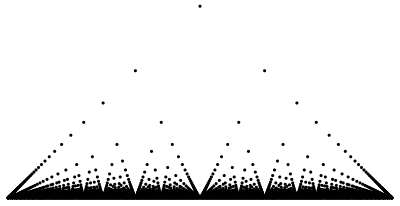
\includegraphics[width=0.5\linewidth]{figure/thomae_function.png}
			\caption{Thomae's Function in the Unit Interval}
		\end{figure}
	\end{example}
	\begin{proposition}
		For every $a \in \R$, $\lim_{x \to a} f(x) = 0$. As a result, $D_f = \Q$.
		\begin{proof}
			WLOG, consider the domain $a \in (0, 1)$ only, show:
			\begin{align}
				\forall \varepsilon > 0\ \exists\ \delta > 0\ s.t.\ \forall x \in V_\delta^o(a),\ f(x) \in V_\varepsilon(0)
			\end{align}
			Fix $\varepsilon > 0$. \\
			Note that there exists $N \in \N$ such that $n \geq N \implies \abs{\frac{1}{n}} < \varepsilon$.\\
			Because $\Q$ is countable, define finite set $L$ following Cantor's diagonal order
			\begin{align}
				L := \left\{
				0, 1, \frac{1}{2},  \frac{1}{3}, \frac{2}{3}, \frac{1}{4}, \frac{3}{4}, \cdots,
				\frac{N-2}{N-1}
				\right \} \backslash \{ a \}
			\end{align}
			That is, $L$ contains every rational number such that its denominator in the lowest form is less than $N$ excluding $a$ (if $a$ is rational). \\
			Define $m := \min_{q_i \in L} \abs{a - q_i}$, which is well-defined because $L$ is finite. \\
			Take $\delta := \frac{m}{2}$, note that $V_\delta (a) \cap \Q \cap L = \varnothing$ by construction. \\
			Let $x \in V_\delta^o(a)$, either \\
			(i) $x \in \Q \implies x \notin L \implies x = \frac{p}{q}$ where $q \geq N$, which implies $f(x) = \frac{1}{q} < \varepsilon$; \\
			(ii) or $x \notin \Q \implies f(x) = 0 < \varepsilon$. \\
			Either case implies the limit to be zero. \\
			Therefore $f$ is discontinuous on $\Q$.
		\end{proof}
	\end{proposition}
	
	\begin{theorem}
		Composition of continuous functions is continuous. \\
		Given $f: A \to \R$, $g: B \to \R$ such that the range $f(A) \subseteq B$. If $f$ is continuous at $c \in A$, and if $g$ is continuous at $f(c) \in B$. Then $g \circ f$ is continuous at $c$.
	\end{theorem}
	
	\begin{proof}
		Let $\varepsilon > 0$, and $g(x)$ is continuous at $f(c)$. 
		\begin{align}
			\exists\ \tilde{\delta}\ s.t.\ f(x) \in V_{\tilde{\delta}}(f(c)) &\implies g \circ f(x) \in V_\varepsilon (g \circ f(x)) \\
			\exists\ \delta > 0\ s.t.\ x \in V_\delta(c) &\implies f(x) \in V_{\tilde{\varepsilon} = \tilde{\delta}} (f(c))
		\end{align}
	\end{proof}
	
	\subsection{Continuous Functions on Compact Sets}
	
	\begin{theorem}
		Let $K$ be a compact set in $\R$, and $f: K \to \R$ is a continuous function, then $f(K)$ is compact.
	\end{theorem}
	
	\begin{proof}
		Let $(y_n) \subseteq K$. Consider $f^{-1}(y_n) \neq \varnothing$, take $x_n \in f^{-1}(y_n)$ to construct a sequence.\\
		Because $K$ is compact, there exists a subsequence of $(x_n)$ converges to $x \in K$.\\
		Since $f$ is continuous, $f(x_n)$ converges to $f(x) \in f(K)$.
	\end{proof}
	
	\begin{theorem}[Extreme Value Theorem]
		If $f: K \to \R$ is continuous on a compact set $K \subset \R$. Then $f$ attains a maximum and minimum value. That is,
		\begin{align}
			\exists\ x_0, x_1 \in K,\ s.t.\ f(x_0) \leq f(x) \leq f(x_1)\ \forall x \in K
		\end{align}
	\end{theorem}
	
	\begin{proof}
		$f(K)$ is compact, in particular it is bounded in $\R$. So it possesses a supremum $\sup f(K)$. \\
		Then there exists a sequence converging to the supremum. 
		Because $f(K)$ is bounded as well, its limit can be attained in $K$. Therefore the maximum is attainable (minimum case is similar).
	\end{proof}
	
	\subsection{Uniform Continuity}
	\begin{example}[Uniformly Continuous]
		$f(x) = 3x + 1$ is continuous for every $c \in \R$.
	\end{example}
	
	\begin{proof}
		Let $\varepsilon > 0$, take $\delta = \frac{\varepsilon}{3}$ gives the definition of continuity. \ul{Note that $\delta$ does not depend on particular $c$.}
	\end{proof}
	
	\begin{example}[Non-uniformly Continuous]
		$y = x^2$ is continuous for every $c \in \R$.
	\end{example}
	
	\begin{proof}
		Let $\varepsilon > 0$, \\
		Note that $\abs{x+c} = \abs{x-c+2c} \leq \abs{x-c} + 2\abs{c}$. \\
		Suppose $\delta \leq 1$ (the following argument works for $x \in V_1(c)$ only):
		\begin{align}
			\abs{x^2 - c^2} &= \abs{x-c}\abs{x+c} \\
			&\leq \delta \abs{x+c} \\
			&\leq \delta (\abs{x-c} + 2\abs{c}) \\
			&\leq \delta(1 + 2 \abs{c}) < \varepsilon
		\end{align}
		Take $\delta := \min \left\{1, \frac{1}{1 + 2 \abs{c}} \right\}$. \ul{Note that $\delta$ depends on particular realization $c$.}
	\end{proof}
	
	\begin{definition}
		A function $f$ is \textbf{uniformly continuous} \ul{on $A \subset \R$} if 
		\begin{align}
			\forall \varepsilon > 0\ \exists \delta > 0\ s.t.\ \forall x, y \in \R\ \abs{x - y} < \delta \implies \abs{f(x) - f(y)} < \varepsilon
		\end{align}
	\end{definition}
	
	\begin{theorem}[Sequential Criterion for Absence of Uniform Continuity]
		Let $f: A \to \R$, the following are equivalent:
		\begin{enumerate}[(i)]
			\item $f$ fails to be uniformly continuous on $A$;
			\item $\exists \varepsilon_0 > 0$ and two sequences $(x_n), (y_n) \subseteq A$ such that $\abs{x_n - y_n} \to 0$ but $\abs{f(x_n) - f(y_n)} \geq \varepsilon_0$ for every $n \in \N$.
		\end{enumerate}
	\end{theorem}

	\begin{proof}
		$f: A \to \R$ is not uniformly continuous, \\
		\ul{iff} $\exists \varepsilon > 0\ s.t.\ \forall \delta > 0\ \exists x, y \in \R\ s.t.\ \abs{x_\delta - y_\delta} < \delta \land \abs{f(x_\delta) - f(y_\delta)} \geq \varepsilon_0$. \\
		For each $n \in \N$, take $\delta = \frac{1}{n}$ and construct two sequences.
	\end{proof}
	
	\begin{example}
		Let $f(x) = \sin(x^{-1})$ defined on $A = (0, 1)$. \\
		Take $x_n := \frac{1}{2n + \frac{\pi}{2}}$ and $y_n = \frac{1}{2n + \frac{3\pi}{2}}$. It is evident that $f(x_n) = 1$ and $f(y_n) = -1$ for every $n \in \N$. By taking $\varepsilon_0 = 2$, the proof is complete.
	\end{example}
	
	\begin{example}
		$f(x) = x^2$ is not uniformly continuous. \\
		Consider two sequences $(x_n) = (n)$ and $(y_n) = \left (n + \frac{1}{n} \right )$. \\
		Note that $\abs{x_n - y_n} = \abs{\frac{1}{n}} \to 0$. \\
		Moreover, $\abs{f(x_n) - f(y_n)} = \abs{2 + \frac{1}{n^2}} > 2$. \\
		Therefore $f$ is not uniformly continuous.
	\end{example}
	
	\begin{theorem}[Uniform Continuity on Compact Set]
		A continuous function fo $f$ on a compact $K$ is uniformly continuous.
	\end{theorem}
	
	\begin{proof}
		Suppose, for contradiction, $f$ is continuous but not uniformly continuous. \\
		Then there exists $\varepsilon_0 > 0$ and $(x_n), (y_n) \subseteq K$ such that $\abs{x_n - y_n} \to 0$ and $\abs{f(x_n) - f(y_n)} \geq \varepsilon_0$. \\
		Because $K$ is compact, there exists subsequences of $(x_n)$ and $(y_n)$ converging to $x, y \in K$. \\
		Suppose $x \neq y$, it contradicts $\abs{x_n - y_n} \to 0$ because this property holds for subsequences as well. \\
		Therefore, $(x_{n_k})$ and $(y_{n_k})$ converge to the same limit. \\
		Because $f$ is continuous, $\lim_{k \to \infty} [f(x_{n_k}) - f(y_{n_k})] = 0 < \varepsilon_0$, contradiction.
	\end{proof}
	
	\subsection{Intermediate Value Theorem}
	\begin{theorem}
		Let $f: [a, b] \to \R$ be a continuous function, if $L \in \R$ such that either
		\begin{enumerate}[(i)]
			\item $L \in (f(a), f(b))$,
			\item or $L \in (f(b), f(a))$.
		\end{enumerate}
		Then $\exists\ c \in (a, b)$ such that $f(c) = L$.
	\end{theorem}
	
	\begin{lemma}
		All the connected subsets of $\R$ are intervals.
	\end{lemma}
	
	\begin{theorem}
		Continuous map preserves connectedness. That is, for some $f: G \to \R$ continuous with $G \subseteq \R$, then $E \subseteq G$ connected $\implies$ $f(E)$ connected.
	\end{theorem}
	
	\begin{proof}
		Suppose $f(E) = A \cup B$, where $A, B \neq \varnothing$ and disjoint. \\
		Note that $E = f^{-1}(A) \cup f^{-1}(B)$ with $f^{-1}(A) \cap f^{-1}(B) = \varnothing$ (evident using contradiction). \\
%		Moreover, $E = f^{-1}(A) \cup f^{-1}(B)$. \\
		Because $E$ is connected, either there exists a convergent sequence in $f^{-1}(A)$ converges to somewhere in $f^{-1}(B)$ or a convergent sequence in $f^{-1}(B)$ converges to somewhere in $f^{-1}(A)$. \\
		WLOG, suppose there exists a sequence $(x_n) \in f^{-1}(A)$ converges to some point $x \in f^{-1}(B)$. \\
		Because $f$ is continuous, $\lim_{n \to \infty} f(x_n) = f(x) \in B$. \\
		That is, there exists sequence $(f(x_n)) \subseteq A$ converges to $f(x) \in B$. \\
		$E$ is connected.
	\end{proof}
	
	\begin{proof}[Proof of IVT.]
		Let $f: [a, b] \to \R$ be a continuous function. \\
		WLOG, suppose $f(a) < f(b)$. \\
		Let $L \in (f(a), f(b))$. \\
		Note that $f([a, b])$ is connected by previous theorem, therefore $f([a, b])$ is an interval by previous lemma. \\
		hence, $f([a, b])$ contains every point between $f(a)$ and $f(b)$, in particular $L$. \\
		Therefore, $\exists\ c \in [a, b]$ with $f(c) = L$. \\
		Note that $f(a), f(b) \neq L$, so $c \neq a, b$. \\
		Therefore, the chosen $c \in (a, b)$.
	\end{proof}
	
	\begin{remark}
		EVT says the continuous functions' image of a compact set is compact. \\
		IVT says the continuous functions' image of a connected set is connected.
	\end{remark}
	
	\begin{definition}
		A function $f$ possesses the \textbf{intermediate value property} on closed interval $[a, b]$ if for every $x < y$ in $[a, b]$ and $f(x) < L < f(y)$, it is always possible to find $c \in (a, b)$ such that $f(c) = L$.
	\end{definition}
	
	\begin{theorem}[IVT restated]
		$f$ is continuous $\implies$ $f$ satisfies IVP.
	\end{theorem}
	
	\begin{remark}
		The converse of IVT is not true. \\
		Consider 
		\begin{align}
			g(x) = \begin{cases}
				\sin \frac{1}{x} &\tx{ if } x \neq 0 \\
				0 &\tx{ if } x = 0
			\end{cases}
		\end{align}
		$g(x): [-1, 1] \to [-1 , 1]$ satisfies IVP, but $g(x)$ is not continuous on $[-1, 1]$, in particular, $g(x)$ is discontinuous at 0.
	\end{remark}
	
	\begin{proposition}
		If a sequence of functions $(f_n)$ converges uniformly to $f$, then $(f_n)$ converges point-wise to $f$ as well.
	\end{proposition}
	
	\begin{example}
		$f_n(x) - \frac{(x^2 + nx)}{n}$ has point-wise limit to $f(x) = x$ but it does not converge uniformly.
	\end{example}
	
	\section{Sequences and Series of Functions}
	\subsection{Sequences of Functions}
	
	\begin{definition}
		For each $n \in \N$, let $f_n$ be a function defined on $A \subseteq \R$. The sequence $(f_n)_{n \in \N}$ \textbf{converges point-wise} on $A$ to a function $f: A \to \R$ if
		\begin{align}
			\forall x \in A, (f_n(x)) \to f(x)
		\end{align}
		That is,
		\begin{align}
			\forall x \in A,\forall \varepsilon > 0\ \exists N_x \in \N\ s.t.\ \forall n \geq N_x,\ f_n(x) \in V_\varepsilon(f(x))
		\end{align}
		\emph{That is, the sequence induced at each $x \in A$ is convergent, and the value of $N_x$ can depend on specific $x$.}
	\end{definition}
	
	\begin{definition}
		Let $(f_n)$ be a sequence of functions defined on $A \subseteq \R$. Then $(f_n)$ \textbf{converges uniformly} on $A$ to $f: A \to \R$ if 
		\begin{align}
			\forall \varepsilon > 0\ \exists N \in \N\ s.t.\ \forall x \in A\ \forall n \geq N,\ f_n(x) \in V_\varepsilon(f(x))
		\end{align}
		\emph{The uniform convergence requires a single $N$ to work for every $x \in A$.}
	\end{definition}
	
	\begin{theorem}[Cauchy Criterion]
		Given a sequence of functions $(f_n)$ defined on $A \subseteq \R$, the following are equivalent:
		\begin{enumerate}[(i)]
			\item $(f_n)$ converges uniformly on $A$;
			\item (\textbf{Uniformly Cauchy})$\forall \varepsilon > 0\ \exists N \in \N\ s.t.\ \abs{f_n(x) - f_m(x)} < \varepsilon\ \forall m, n \geq N, \forall x \in A$.
		\end{enumerate}
	\end{theorem}
	
	\begin{proof}
		($\implies$)\\
		The sufficient condition is immediate by triangle inequality. \\
		Suppose $(f_n) \overset{unif}{\to} f$, let $\varepsilon > 0$, take $N \in \N$ such that $\forall n \geq N, \abs{f_n(x) - f(x)} < \frac{\varepsilon}{2}$ for every $x \in A$. \\
		Take the same $N$ and let $m, n \geq N$, let $x \in A$,
		\begin{align}
			\abs{f_n(x) - f_m(x)} &= \abs{f_n(x) - f(x) + f(x) - f_m(x)} \\
			&\leq \abs{f_n(x) - f(x)} + \abs{f(x) - f_m(x)} \\
			&<\varepsilon
		\end{align} \\
		($\impliedby$) \\
		Assume $(f_n)$ is uniformly Cauchy. \\
		Let $\varepsilon > 0$. \\
		$\forall x \in A$, $(f_n(x))_{n \in \N}$ is a Cauchy sequence in $\R$. \\
		By the completeness of $\R$, $(f_n(x)) \to f(x)$ for some point-wise limit $f(x)$. \\
		We are going to show $(f_n)$ converges uniformly to the point-wise limit. \\
		By uniform Cauchy, $\exists N \in \N$ such that $\forall m \geq N$, $n = m+k \geq N$, and $\forall x \in A$,
		\begin{align}
			\abs{f_m(x) - f_n(x)} < \frac{\varepsilon}{2}
		\end{align}
		Fix $x \in A$,
		\begin{align}
			f(x) &= \lim_{n \to \infty} f_n(x) \\
			\implies \abs{f_m(x) - f(x)} &= \lim_{n \to \infty} \abs{f_m(x) - f_n(x)} \\
			&= \lim_{k \to \infty} \abs{f_m(x) - f_{m+k}(x)} \\
			&\leq \frac{\varepsilon}{2} < \varepsilon \tx{ (order limit theorem)}
		\end{align}
	\end{proof}
	
	\begin{theorem}[Continuous Limit Theorem]
		Let $(f_n)$ be a sequence of functions defined on $A \subseteq \R$ that \ul{converges uniformly} on $A$ to a function $f$. If each $f_n$ is continuous at $c \in A$, then $f$ is continuous at $c$.
	\end{theorem}
	
	\begin{proof}
		Let $(f_n)$ be a sequence of continuous functions, let $c \in A$, note that for arbitrary $N \in \N$, 
		\begin{align}
			\abs{f(x) - f(c)} &= \abs{f(x) - f_N(x) + f_N(x) - f_N(c) + f_N(c) - f(c)} \\
			&\leq \abs{f(x) - f_N(x)} + \abs{f_N(x) - f_N(c)} + \abs{f_N(c) - f(c)}
		\end{align}
		Where the last term can be made arbitrarily small given the uniform convergence property of $(f_n)$. And the first two terms can be made arbitrarily small as well given the continuity properties. \\
		This concludes the continuity of $f$. 
	\end{proof}
	
	\begin{theorem}[Differentiable Limit Theorem]
		Let $(f_n) \to f$ \ul{pointwise} on closed interval $[a, b]$, and assume that each $f_n$ is differentiable.
		If $(f'_n) \to g$ \ul{uniformly} on $[a, b]$, then the limit $f$ is differentiable and $f' = g$.
	\end{theorem}
	
	\begin{proof}
		Let $c \in [a, b]$, note that 
		\begin{align}
			f'(c) &= \lim_{x \to c} \frac{f(x) - f(c)}{x - c}
		\end{align}
		The following holds for every $n \in \N$:
		\begin{align}
			&\quad\abs{\frac{f(x) - f(c)}{x - c} - g(c)} \\
			&=\abs{\frac{f(x) - f(c)}{x - c} - \frac{f_n(x) - f_n(c)}{x - c} + \frac{f_n(x) - f_n(c)}{x - c} - f'_n(c) + f'_n(c) - g(c)} \\
			&\leq \abs{\frac{f(x) - f(c)}{x - c} - \frac{f_n(x) - f_n(c)}{x - c}} + \abs{\frac{f_n(x) - f_n(c)}{x - c} - f'_n(c)} + \abs{f_n'(c) - g(c)}
		\end{align}
		In particular, one may choose $N_1 \in \N$ such that 
		\begin{align}
			\abs{f'_n(c) - g(c)} < \frac{\varepsilon}{3}	
		\end{align}
		for every $n \geq N_1$. \\
		Moreover, given the Cauchy property of uniform convergence, there exists $N_2 \in \N$ such that $\forall m, n \geq N_2$, $\abs{f'_m(x) - f'_n(x)} < \frac{\varepsilon}{3}$ for every $x \in A$. \\
		Define $N = \max\{N_1, N_2\}$.\\
		Note that $\exists\ \delta > 0$ such that 
		\begin{align}
			x \in V^o_\delta(c) \implies \abs{\frac{f_N(x) - f_N(c)}{x - c} - f'_N(c)} < \frac{\varepsilon}{3}
		\end{align}
		Let $m \geq N$, for an arbitrary $x \in V^o_\delta(c)$, WLOG, suppose $x < c$. Applying the mean value theorem on $f_m - f_N$ gives
		\begin{align}
			f'_m(\eta) - f'_N(\eta) &= \frac{f_m(c) - f_N(c) - [f_m(x) - f_N(x)]}{c-x} \\
			\implies \frac{\varepsilon}{3} > \abs{f'_m(\eta) - f'_N(\eta)} &= \abs{
			\frac{f_m(c) - f_m(x)}{c-x} - \frac{f_N(c) - f_N(x)}{c-x}
			} \\
			\implies \lim_{m \to \infty} \abs{
			\frac{f_m(c) - f_m(x)}{c-x} - \frac{f_N(c) - f_N(x)}{c-x}
			} &= \abs{
			\frac{f(c) - f(x)}{c-x} - \frac{f_N(c) - f_N(x)}{c-x}
			} \\
			&\leq \frac{\varepsilon}{3} \tx{ (order limit theorem)}
		\end{align}
		Therefore, for every $x \in V_\delta^0(c)$, 
		\begin{align}
			\abs{\frac{f(x) - f(c)}{x - c} - g(c)} < \varepsilon
		\end{align}
	\end{proof}
	
	\begin{theorem}
		Let $(f_n)$ be a sequence of \ul{differentiable} functions defined on the closed interval $[a, b]$, and assume $(f'_n)$ \ul{converges uniformly} on $[a, b]$. If there exists a point $x_0 \in [a, b]$ where $f_n(x_n)$ converges, then $(f_n)$ \ul{converges uniformly} on $[a, b]$.
	\end{theorem}
	
	\begin{theorem}[Stronger Version]
		Let $(f_n)$ be a sequence of \ul{differentiable} functions defined on the closed interval $[a, b]$, and assume $(f'_n)$ converges uniformly to a function $g$ on $[a, b]$. \\
		If there exists a point $x_0 \in [a, b]$ for which $f_n(x_0)$ converges, then $(f_n)$ converges uniformly, \\
		Furthermore, the limit function $f$ is differentiable and satisfies $f' = g$.
	\end{theorem}
	
	\subsection{Series of Functions}
	\begin{definition}
		A series of function $\sum_{i=1}^\infty f_n(x)$ converges point-wise/uniformly if $\sum_{i=1}^k f_n(x)$ converges point-wise/uniformly.
 	\end{definition}
 	
 	\begin{example}
 		Note that $\sum_{i=1}^\infty \frac{\sin(nx)}{n^2}$ converges uniformly.
 		\begin{align}
 			\abs{\sum_{i=1}^k \frac{\sin(nx)}{n^2} - \sum_{i=1}^\ell \frac{\sin(nx)}{n^2}} \leq \sum_{n=\ell+1}^k \frac{1}{n^2} < \varepsilon
 		\end{align}
 		Hence, uniformly Cauchy.
 	\end{example}
 	
 	\begin{theorem}
 		If $f_n: S \subseteq \R^k \to \R^m$ continuous, then if $\sum_{n=1}^\infty f_n \to f$ uniformly, then $f$ is also continuous.
 	\end{theorem}
 	
 	\begin{definition}
 		Let $f_k: S \to \R^m$, then $(f_k)$ is \textbf{uniformly Cauchy} on $S$ if 
 		\begin{align}
 			\forall \varepsilon > 0\ \exists N \in \N\ s.t.\ \sup_{x \in S} \norm{\sum_{i=k+1}^\ell f_i(x)} \leq \varepsilon\ \forall \ell > k \geq N
 		\end{align}
 	\end{definition}
 	
 	\begin{theorem}
 		$(f_k)$ is uniformly Cauchy $\iff$ $\sum f_k \to f$ uniformly. \\
 		\emph{This is the same as the theorem mentioned in previous section. Simply define $g_n := \sum_{i=1}^ns f_i(x)$, and $(g_n)$ is uniformly Cauchy if and only if it converges to $g_\infty \equiv \sum_{n=1}^\infty f_n(x)$ uniformly.}
 	\end{theorem}
 	\begin{proof}
 		($\impliedby$)\\
 		Let $g_m := \sum_{k=1}^m f_k(x)$, suppose $g_k \to f$ uniformly. Then, 
 		\begin{align}
 			\forall \varepsilon > 0\ \exists N \in \N\ s.t.\ \abs{g_k - f} < \frac{\varepsilon}{2}\ \forall k \geq N, \forall x \in S
 		\end{align}
 		For every $k > \ell \geq N$,
 		\begin{align}
 			\abs{g_k - g_\ell} \leq \abs{g_k - f} + \abs{f - g_\ell} < \varepsilon\ \forall x \in S
 		\end{align}
 		Therefore, $(f_k)$ is uniformly Cauchy. \\
 		($\implies$) \\
 		Suppose $f(f_k)$ is uniformly Cauchy. Then for every fixed $x \in S$, $(g_k(x))$ is Cauchy. \\
 		So $f(x) = \lim_{k \to \infty} g_k(x)$ exists.
 		\begin{align}
 			&\forall \varepsilon > 0\ \exists N \in \N\ s.t.\ \abs{g_k(x) - g_\ell(x)} < \varepsilon\ \forall k > \ell \geq N,\forall x \in S \\
 			&\implies \abs{f(x) - g_k(x)} = \lim_{\ell \to \infty} \abs{g_\ell(x) - g_k(x)} \leq \varepsilon\ \forall x \in S\\
 			&\implies g_k \to f \tx{ uniformly}
 		\end{align}
 	\end{proof}
 	
 	\begin{theorem}[Term-by-term Continuity Theorem]
 		Let $f_n$ be continuous functions defined on a set $A \subseteq \R$, suppose $\sum^\infty_{n=1} f_n \to f$ \ul{uniformly}, then $f$ is continuous on $A$.
 	\end{theorem}
 	
 	\begin{theorem}[Term-by-term Differentiability Theorem] 
 		Let $f_n$ be continuous functions defined on $A \subseteq \R$, and suppose
 		\begin{enumerate}[(i)]
 			\item $\sum^\infty_{n=1} f'_n \to g$ \ul{uniformly};
 			\item There exists a point $x_0$ such that the series converges at $x_0$.
 		\end{enumerate}
 		Then, $\sum^\infty_{n=1} f_n \to f$ converges \ul{uniformly} to a differentiable function $f$ with $f'(x) = g(x)$.\\
 		That is
 		\begin{align}
 			f(x) &= \sum_{n=1}^\infty f_n(x) \\
 			f'(x) &= \sum_{n=1}^\infty f'_n(x)
 		\end{align}
 	\end{theorem}
 	
 	\begin{theorem}[Weierstrass M-test]
 		Let $a_n: S \to \R^m$, and sequence $M_n \in \R$. If
 		\begin{align}
 			\exists N \in \N\ \forall k \geq N\ \sup_{x \in S} \abs{a_n(x)} \leq M_n
 		\end{align}
 		then $\sum_{n=1}^\infty M_n$ \ul{converges} implies $\sum_{n=1}^\infty a_n$ \ul{converges uniformly}.
 	\end{theorem}
 	
 	\begin{proof}
 		The desired result can be shown by showing the sequence of partial sums is Cauchy. \\
 		Let $\varepsilon > 0$, show that there exists $k \in \N$ such that
 		\begin{align}
 			\forall m, n \geq k,\quad \abs{S_m(x) - S_n(x)} < \varepsilon
 		\end{align}
 		WLOG, suppose $m > n$, then 
 		\begin{align}
 			\abs{S_m(x) - S_n(x)} &= \abs{a_{n+1}(x) + \cdots a_m(x)} \\
 			&\leq \abs{M_{n+1} + \cdots + M_n}
 		\end{align}
 	\end{proof}
 	
 	\begin{proof}
 		\begin{align}
 			\forall x \in S \sum_{n=1}^\infty \abs{a_n(x)} &\leq \sum_{n=1}^\infty \sup_{x \in S} \abs{a_n(x)} \\
 			&\leq \sum_{n=1}^N \sup_{x \in S} \abs{a_n(x)} + \sum_{n=N+1}^\infty M_n < \infty
 		\end{align}
 		Therefore, $f(x) = \sum_{n=1}^\infty a_n(x)$ exists. \\
 		Note that $\forall x \in S, \forall \ell \geq N$:
 		\begin{align}
 			\abs{f(x) - \sum_{k=1}^\ell a_k(x)} &= \abs{\sum_{k = \ell + 1}^\infty a_k(x)}  \\
 			&\leq \sum_{k=\ell+1}^\infty \abs{a_n(x)} \\
 			&\leq \sum_{k=\ell+1}^\infty M_k < \infty \\
 			\implies \lim_{\ell \to \infty} \sup_{x \in S} \abs{f(x) - \sum_{k=1}^\ell a_k(x)} &\leq \lim_{\ell \to \infty} \sum_{k=\ell+1}^\infty M_n = 0
 		\end{align}
 		Therefore $\sum a_k \to f$ uniformly.
 	\end{proof}
 	
 	\begin{example}
 		Consider $\sum \frac{x^n}{n!}$ defined on $x \in [-A, A]$. Note that
 		\begin{align}
 			\sup_{x \in S} \abs{\frac{x^n}{n!}} &\leq \frac{A^n}{n!} =: M_n
 		\end{align}
 		By ratio test, $\sum M_n$ converges. \\
 		By M-test $\sum \frac{x^n}{n!}$ converges uniformly on $[-A, A]$. \\
 		Therefore, $\sum \frac{x^n}{n!}$ is continuous on $[-A, A]$.
 	\end{example}
 	
 	\begin{example}[Geometric Series]
 		\begin{align}
 			\sum_{n=1}^\infty (-x^2)^n
 		\end{align}
 		By ratio test, the series converges only on $(-1 ,1)$. In particular, it converges to $\frac{1}{1 + x^2}$. \\
 		For every $0 < r < 1$, for $x \in [-r, r]$, then 
 		\begin{align}
 			\sup_{x \in [-r, r]} \abs{(-x^2)^n} = r^{2n}
 		\end{align}
 		and $\sum_{n=1}^\infty r^{2n} = \frac{1}{1+r^2}$ implies $\sum_{n=1}^\infty (-x^2)^n$ converges uniformly on $[-r, r]$.
 	\end{example}
 	
 	\begin{example}[Weierstrass Function]
 		Define
 		\begin{align}
 			f(x) = \sum_{n=1}^\infty \underbrace{\frac{1}{2^n} \cos(10^n \pi x)}_{f_n(x)}
 		\end{align}
 		Note that $\sup_{x \in S} \abs{f_n(x)} \leq \frac{1}{2^n}$, and $\sum_{n=1}^\infty \frac{1}{2^n} \to 1$. Therefore, $\sum f_n \to f$ uniformly on $\R$, so that $f$ is continuous.
 	\end{example}
 	\begin{proposition}
 		$f$ is nowhere differentiable.
 	\end{proposition}
 	\begin{proof}
 		Let $x \in \R$ with decimal expansion $x_0\cdot x_1 x_2 \cdots$. \\
 		Construct sequence $(z_n) \to x$ as following: \\
		Fix $n$, let $y_0 = x_0.x_1 \cdot x_n$ and $y_1 = y_0 + \frac{1}{10^n}$. \\
		Note that $10^n \pi y_i$ is an integer multiplied by $\pi$, which implies $f(y_0) = \frac{(-1)^{x_n}}{2^n}$, $f(y_1) = \frac{(-1)^{x_{n+1}}}{2^n}$
 		such that
 		\begin{align}
 			\abs{\frac{f(z_n) - f(x)}{z_n - x}} \to \infty
 		\end{align}
 	\end{proof}
 	
 	\begin{example}
 		Let
 		\begin{align}
 			h(x) &:= \sum_{n=1}^\infty \frac{1}{x^2 + n^2} \equiv \sum_{n=1}^\infty h_n(x)
 		\end{align}
 		Claim: $h(x)$ is continuous and differentiable on $\R$.
 	\end{example}
 	
 	\begin{proof}[Continuity]
 		Note that each $h_n(x)$ is continuous, so is each partial sum $S_k := \sum_{n=1}^k h_n(x)$. \\
 		By Weierstrass M-test, each $\abs{h_n(x)} \leq \frac{1}{n^2} \equiv M_n$, the series converges to $h(x)$ uniformly. \\
 		Therefore, by the definition of series convergence, the sequence of partial sums, in which all elements are continuous, converges uniformly to $h(x)$, hence $h(x)$ is continuous as well. 
 	\end{proof}
 	
 	\begin{proof}[Differentiability]
 		We've already shown the sequence of partial sum converges uniformly to $h(x)$. \\
 		All we need to show is the derivative of partial sums converges uniformly to some function. \\
 		Equivalently, we are showing the uniform convergence of series of derivatives. \\
 		In particular,
 		\begin{align}
 			h_n'(x) &= -\frac{2x}{(x^2 + n^2)^2} \\
 			S'_k(x) &= \sum_{n=1}^k h_n'(x) = - \sum_{n=1}^k \frac{2x}{(x^2 + n^2)^2}
 		\end{align}
 		Apply M-Test again,
 		\begin{align}
 			\abs{h_n'(x)} &= \abs{-\frac{2x}{(x^2 + n^2)^2}} \\
 			&= \frac{2}{\frac{x^2+n^2}{x}(x^2+n^2)} \\
 			&= \frac{2}{(x + \frac{n^2}{x})(x^2 + n^2)}
 		\end{align}
 		Note that 
 		\begin{align}
 			\left(\sqrt{x} - \frac{n}{\sqrt{x}} \right)^2 = x - 2n + \frac{n^2}{x} \geq 0 \\
 			\implies \left(x + \frac{n^2}{x} \right) \geq 2n
 		\end{align}
 		Therefore,
 		\begin{align}
 			\abs{h_n'(x)} &\leq \frac{2}{2n(x^2 + n^2)} \\
 			&\leq \frac{1}{n^3}
 		\end{align}
 		Therefore,
 		\begin{align}
 			\sum_{n=1}^\infty h'_n(x) \to g(x) \tx{ uniformly}
 		\end{align}
 		Hence, $h(x)$ is differentiable, in particular, $h'(x) = g(x)$.
 	\end{proof}
 	
 	\subsection{Power Series}
 	\begin{definition}
 		A \textbf{power series} takes the form of 
 		\begin{align}
 			f(x) &= \sum_{n=0}^\infty a_n x^n
 		\end{align}
 		in which $f(0) < \infty$ trivially.
 	\end{definition}
 	
 	\begin{theorem}
 		If a power series converges at some point $x_0 \in \R$, then it it converges absolutely for any $x$ such that $\abs{x} \leq \abs{x_0}$. \todo{verify the inequality, strictly?}
 	\end{theorem}
 	
 	\begin{proof}
 		The result can be easily established via comparison test. \\
 		Suppose $f(x_0)$ converges, let $x \in \overline{V}_{\abs{x_0}}(0)$. \\
 		By the convergence of $f(x_0)$, $(a_n x_0^n) \to 0$, so that $\abs{a_n x_0^n} \leq M\ \forall n \in \N$.
 		\begin{align}
 			\abs{a_n x^n} &= \abs{a_n} \abs{\frac{x^n}{x_0^n} x_0^n} \\
 			&= \abs{a_n x_0^n} \abs{\frac{x}{x_0}}^n \\
 			&\leq M \abs{\frac{x}{x_0}}^n 
 		\end{align}
 		In which $\sum_{n=0}^\infty M \abs{\frac{x}{x_0}}^n$ converges as a power series with ratio less than 1. \\
 		Therefore, $\sum_{n=0}^\infty a_n x^n$ is convergent by comparison test.
 	\end{proof}
 	
 	\begin{definition}
 		\textbf{Radius of convergence} and \textbf{interval of convergence}
 		\todo{Do we need to define this?}
 	\end{definition}
 	
 	\begin{theorem}[Abel's Theorem]
 		Suppose $g(x) = \sum_{n=0}^\infty a_n x^n$ converge somewhere $x = R > 0$, then $g(x)$ converges uniformly (as a series of functions) on $[0, R]$. \\
 		The same holds for $-R$: if $g(-R)$ converges, then $g(x)$ converges uniformly on $[-R, 0]$.
 	\end{theorem}
 	
 	\begin{theorem}
 		If a power series $g(x) = \sum_{n=0}^\infty a_n x^n$ converges point-wisely on $A \subseteq \R$, then it converges uniformly on any compact subset $K \subseteq A$.
 	\end{theorem}
 	
 	\begin{proof}
 		\todo{Complete this proof.}
 	\end{proof}
  	
 	\newpage
 	\section{Appendix: Miscellaneous}
 	\begin{proposition}[Midterm 1, Q7]
 		Let $(a_n)$ be a bounded sequence,\\
 		let $S:= \{x \in \R: x < a_n \tx{ for infinitely many terms }a_n\}$. \\
 		Then $\exists (a_{n_k}) \to s := \sup S$.
 	\end{proposition}
 	
 	\begin{lemma}
 		$S$ is bounded above, therefore $s := \sup S$ is well-defined.
 	\end{lemma}
 	\begin{proof}
 		Every element in $S$ is bounded from above by infinitely many elements from $(a_n)$, which are themselves bounded. Therefore $S$ is bounded from above. \\
 		So $s$ is well-defined by the completeness axiom.
 	\end{proof}
 	
 	\begin{proof}[Proof. Case 1]
 		Suppose there are infinitely many $a_n > s$. \\
 		Then either $\forall k \in \N\ \exists a_{n_k} \in [s, s + \frac{1}{k})$, such subsequence $(a_{n_k}) \to s$. \\
 		Or $\exists k \in \N$ such that no $a_n$ in $[s, s + \frac{1}{k})$, this leads to a contradiction to the assumption that $s$ is the least upper bound.
 	\end{proof}
 	
 	\begin{proof}[Proof. Case 2]
 		Suppose there are only finitely many $a_n > s$. \\
 		Consider $(s - \frac{1}{k}, s]$, by the definition of supremum, $\forall k \in \N,\ \exists s_k \in (s - \frac{1}{k}, s] \cap S$. \\
 		But $s_k < a_n$ for infinitely many $a_n$ by definition of $S$. \\
 		In particular, because there are only finitely many $a_n > s$, there must be infinitely many $a_n$ clustered in $(s - \frac{1}{k}, s]$ for every $k \in N$.\\
 		For each $k \in \N$, one can pick $a_{n_k} \in (s - \frac{1}{k}, s]$ and $(a_{n_k}) \to s$.
 	\end{proof}
 	
 	\begin{proposition}[Another Midterm Question]
 		The open clopen set in $\R$ is $\varnothing$ and $\R$.
 	\end{proposition}
 	
 	\begin{proof}
 		Suppose, for contradiction, there exists $U, V \neq \varnothing$ and $V = U^c$, further $U$ is clopen. \\
 		By definition of closedness and openness, $V$ is clopen as well. \\
 		Pick $a \in U$ and $b \in V$. WLOG, assume $a < b$. \\
 		Construct $X \subseteq U$ as
 		\begin{align}
 			X := \{x \in U: x < b\}
 		\end{align}
 		$X$ is nonempty because $a \in X$.\\
 		$X$ is certainly bounded above by $b$, hence, by the completeness axiom, $\exists\ \alpha = \sup X$. \\
 		\textbf{Calim:} $\alpha \in \partial U$.\\
 		By the definition of supremum, for every $\varepsilon > 0$, 
 		\begin{align}
 			\forall \varepsilon > 0,\ V_\varepsilon(\alpha) \cap X \neq \varnothing \\
 			\implies V_\varepsilon(\alpha) \cap U \neq \varnothing
 		\end{align}
 		\emph{Case 1:} \\
 		If $V_\varepsilon(\alpha) \cap V = \varnothing$ for some $\varepsilon > 0$, then $V_\varepsilon(\alpha) \subseteq U$. \\
 		\emph{Subcase 1:} \\
 		If $\alpha + \frac{\varepsilon}{2} \leq b$, then $\alpha \neq \sup X$ (contradiction); \\
 		\emph{Subcase 2:} \\
 		If $\alpha + \frac{\varepsilon}{2} > b$, then $b \in V_{\varepsilon/2}(\alpha) \cap V \subseteq V_\varepsilon(\alpha) \cap V = \varnothing$ (contradiction).\\
 		\emph{Case 2:}
 		$\forall \varepsilon > 0,\ V_\varepsilon(\alpha) \cap V \neq \varnothing$, then by definition, $\alpha \in \partial U \subseteq U$ and $\alpha \in \partial U \subseteq U$ because $U$ and $V$ are closed. \\
 		This leads to a contradiction that $U \cap V = \varnothing$.
 	\end{proof}
 	
 	\begin{proposition}[Sample Midterm 2]
 		Let $\mc{K} = \{K_\lambda: \lambda \in \Lambda \}$ be a collection of compact subsets of $\R$ such that the intersection of every finite sub-collection is nonempty. Then $\bigcap_{\lambda \in \Lambda} K_\lambda \neq \varnothing$.
 	\end{proposition}
 	
 	\begin{proof}
 		Suppose, for contradiction, $\bigcap_{\lambda \in \Lambda} K_\lambda = \varnothing$. \\
 		Take an arbitrary $K_0 \in \mc{K}$, which is obviously non-empty. \\
 		Then,
 		\begin{align}
 			K_0 &= K_0 \cap \varnothing^c \\
 			&= K_0 \cap \left(\bigcap_{\lambda \in \Lambda} K_\lambda\right)^c \\
 			&= K_0 \cap \bigcup_{\lambda \in \Lambda} K_\lambda^c \\
 			&= \bigcup_{\lambda \in \Lambda} K_0 \cap K_\lambda^c
 		\end{align}
 		For an arbitrary $\lambda \in \Lambda$, let $x \in K_0 \cap K_\lambda^c \neq \varnothing$. \\
 		Because $K_\lambda^c$ is open in $\R$, $\exists\ V_\varepsilon(x) \subseteq K_\lambda^c$. \\
 		Note that because $K_\lambda^c$ is open in $\R$, therefore $K_0 \cap K_\lambda^c$ is open in $K_0$. \\
 		Hence, $\bigcup_{\lambda \in \Lambda} K_0 \cap K_\lambda^c$ is an open cover of $K_0$. The compactness of $K_0$ suggests it has a finite subcover, say $\bigcup_{\lambda=1}^n K_0 \cap K_\lambda^c$. That is,
 		\begin{align}
 			K_0 &= \bigcup_{\lambda=1}^n K_0 \cap K_\lambda^c \\
 			&= K_0 \cap \bigcup_{\lambda=1}^n K_\lambda^c \\
 			&= K_0 \backslash \bigcap_{\lambda=1}^n K_\lambda \\
 			\implies &\bigcap_{\lambda=1}^n K_\lambda = \varnothing
 		\end{align}
 		$\contradiction$
 	\end{proof}
\end{document}












